\documentclass[11pt,final]{amsart}%default 10pt
%prepared in AMSLaTeX, under LaTeX2e

\usepackage[total={6.2in,9.0in},top=1.2in,left=1.1in]{geometry}

\usepackage{natbib}

\usepackage{amssymb,alltt,verbatim,xspace,fancyvrb,color,empheq}
\usepackage{palatino}
\usepackage[sc]{mathpazo}
\usepackage[T1]{fontenc}

% check if we are compiling under latex or pdflatex
\ifx\pdftexversion\undefined
  \usepackage[final,dvips]{graphicx}
\else
  \usepackage[final,pdftex]{graphicx}
\fi

% hyperref should be the last package we load
\usepackage[pdftex,
                colorlinks=true,
                plainpages=false, % only if colorlinks=true
                linkcolor=blue,   % only if colorlinks=true
                citecolor=black,   % only if colorlinks=true
                urlcolor=magenta     % only if colorlinks=true
]{hyperref}

\newcommand{\normalspacing}{\renewcommand{\baselinestretch}{1.05}\tiny\normalsize}
\newcommand{\tablespacing}{\renewcommand{\baselinestretch}{1.0}\tiny\normalsize}
\normalspacing

\definecolor{myblue}{rgb}{.8, .8, 1}

\newcommand*\mybluebox[1]{%
\colorbox{myblue}{\hspace{1em}#1\hspace{1em}}}

% math macros
\newcommand\bv{\mathbf{v}}
\newcommand\bV{\mathbf{V}}
\newcommand\bq{\mathbf{q}}
\newcommand\bQ{\mathbf{Q}}

\newcommand\CC{\mathbb{C}}
\newcommand{\DDt}[1]{\ensuremath{\frac{d #1}{d t}}}
\newcommand{\ddt}[1]{\ensuremath{\frac{\partial #1}{\partial t}}}
\newcommand{\ddx}[1]{\ensuremath{\frac{\partial #1}{\partial x}}}
\newcommand{\ddy}[1]{\ensuremath{\frac{\partial #1}{\partial y}}}
\newcommand{\ddxp}[1]{\ensuremath{\frac{\partial #1}{\partial x'}}}
\newcommand{\ddz}[1]{\ensuremath{\frac{\partial #1}{\partial z}}}
\newcommand{\ddxx}[1]{\ensuremath{\frac{\partial^2 #1}{\partial x^2}}}
\newcommand{\ddyy}[1]{\ensuremath{\frac{\partial^2 #1}{\partial y^2}}}
\newcommand{\ddxy}[1]{\ensuremath{\frac{\partial^2 #1}{\partial x \partial y}}}
\newcommand{\ddzz}[1]{\ensuremath{\frac{\partial^2 #1}{\partial z^2}}}
\newcommand{\Div}{\nabla\cdot}
\newcommand\eps{\epsilon}
\newcommand{\grad}{\nabla}
\newcommand{\ihat}{\mathbf{i}}
\newcommand{\ip}[2]{\ensuremath{\left<#1,#2\right>}}
\newcommand{\jhat}{\mathbf{j}}
\newcommand{\khat}{\mathbf{k}}
\newcommand{\nhat}{\mathbf{n}}
\newcommand\lam{\lambda}
\newcommand\lap{\triangle}
\newcommand\Matlab{\textsc{Matlab}\xspace}
\newcommand\RR{\mathbb{R}}
\newcommand\vf{\varphi}

\newcommand{\Wlij}{W^l_{i,j}}
\newcommand{\Wij}{W_{i,j}}
\newcommand{\Plij}{P^l_{i,j}}
\newcommand{\Pij}{P_{i,j}}
\newcommand{\Ylij}{Y^l_{i,j}}
\newcommand{\Yij}{Y_{i,j}}
\newcommand{\upp}[3]{\big<#1\big|_{#3}\,#2\big>}

\newcommand{\Nbreen}{Nordenski\"oldbreen\xspace}


\title[]{A diffusive-closure model of subglacial hydrology}

\author[]{Ward van Pelt and Ed Bueler}


\begin{document}
\scriptsize \hfill \today \normalsize
\vspace{0.5in}

\maketitle
\thispagestyle{empty}

\section{Introduction}

Any reasonable dynamical model of the subglacial aquifer (liquid water layer) under a glacier or ice sheet has at least these two elements: the mass of the water is conserved and the water flows from high to low hydraulic potential.  Physical processes also control the geometry of the aquifer, including the opening of cavities by sliding of the overlying ice past bedrock bumps (i.e.~cavitation) and the closure of cavities and channels by creep.  These physical processes should combine to determine the local relationship between water amount and water pressure.  

This paper describes such a model for distributed systems of linked cavities.  These cavities open by sliding of the ice and they close by ice creep.  Channels are not included in the model.  Wall melt is included as a contribution to the mass conservation equation but not in the cavity evolution equation.

We model water pressure using a damped approximation of a full-cavity formulation of a distributed system \cite{Schoofetal2012}.  In our model pressure is determined non-locally over each connected component of the hydrological system.  However, unlike the \cite{Schoofetal2012} model in which an elliptic variational inequality for pressure must be solved at each time step, we avoid solving an instantaneous distributed balance by not exactly enforcing the full-cavity condition.  Our model replaces the elliptic pressure description by a parabolic approximation.


\section{Elements of a subglacial hydrology continuum model}

We consider a layer of water with thickness $W(t,x,y)$.  This thickness is only meaningful compared to observations if it is regarded as an average over a horizontal scale of tens to thousands of meters \citep{FlowersClarke2002_theory}.  As the hydrologic system has fine spatial variation which one is unable to model with cells of kilometer size, we only attempt to model such spatially-averaged versions of water amount and water pressure.

We assume that water is incompressible and of constant density.  Thus the thickness of the water layer tells us its mass.  Choosing to model subglacial hydrology using a water thickness is not a significant restriction on the physics.  Specific aquifer physics comes from choosing a form for the water flux and a closure for pressure.


\subsection*{Mass conservation}  Suppose $\bq$ is the vector water flux (units $\text{m}^2\,\text{s}^{-1}$) and $\Phi$ is a source term ($\text{m}\,\text{s}^{-1}$).  In two spatial dimensions the mass conservation equation is \citep{Clarke05}
\begin{equation} \label{eq:conserve}
\frac{\partial W}{\partial t} + \Div \bq = \Phi
\end{equation}
We always assume the water thickness is nonnegative:
\begin{equation}
W \ge 0.
\end{equation}

We might separate the water sources between the melt on the lower surface of the glacier versus englacial and/or supraglacial drainage:
\begin{equation}
\Phi = \rho_w^{-1} \left(m + S\right).  \label{drainagesplit}
\end{equation}
Here $\rho_w$ is the density of fresh liquid water, $m$ is the rate at which basal melting (refreeze) of ice adds (removes) water, and $S$ is the rate at which surface runoff or englacial drainage adds water.  For the \Nbreen, Svalbard example below we will take $m=0$ so that in fact only supraglacial drainage input is modeled.


\subsection*{Hydraulic potential and Darcy flow}  The water flux $\bq$ in equation \eqref{eq:conserve} is related to the gradient of a hydraulic potential (head) $\psi(t,x,y)$.  This quantity combines the actual subglacial water pressure $P(t,x,y)$ and the gravitational potential of the top of the water layer,
\begin{equation} \label{eq:potential}
\psi = P + \rho_w g\, (b+W).
\end{equation}
Here $\rho_w$ is the water density ($\text{kg}\,\text{m}^{-3}$), $g$ is the acceleration of gravity ($\text{m}\,\text{s}^{-2}$), and $z=b(x,y)$ ($\text{m}$) is the bedrock elevation, which for simplicity is time-independent.

We have added the term ``$\rho_w g W$'' to the standard hydraulic potential formula \citep[e.g.]{Clarke05} for the reason that is given by \cite{Hewittetal2012}, namely that it is correct.  In fact, differences in the potential at the \emph{top} of the water layer determine the driving potential gradient.  The term is important when considering local minima of the hydraulic potential, where subglacial lakes of finite (not infinitesimal) extent and finite (not infinite) depth should form.  As we will see, this term makes the mass conservation equation diffusive, though the diffusion is only significant when the water depth becomes substantial ($W\gg 1$).

Water flows from high to low hydraulic potential.  The simplest applicable expression of this property is a Darcy flux model for a water sheet following \cite{Clarke05}, namely
\begin{equation}  \label{eq:flux}
\bq = - \frac{K(W) \, W}{\rho_w g} \grad \psi
\end{equation}
Here $K(W)\ge 0$ is the effective hydraulic conductivity ($\text{m}\,\text{s}^{-1}$) which is a continuously-differentiable and increasing function of the water depth $W$.  Both the simplest case $K(W)=K_0$ (constant) and a nontrivial form for $K(W)$ will be considered in this paper.  Even if $K(W)=K_0$ is constant, the flux is larger for a given head gradient when either the ability of the subglacial material to conduct water is bigger (i.e.~$K_0$ is larger) or the water sheet is thicker ($W$ is larger).

Alternatively to equation \eqref{eq:flux}, we could follow \cite{Schoofetal2012} and take
\begin{equation}  \label{eq:fluxalt}
\bq = - \,\tilde k\, W^\alpha\, |\grad \psi|^{\beta-2} \grad \psi
\end{equation}
for $\alpha> 1$, $\beta>1$, and some positive coefficient $\tilde k$.  This more nonlinear form is justified as an instance of a Manning or Darcy-Weisbach law.  Note that \eqref{eq:flux} with $K(W)=\tilde k$ is the $\alpha=1,\beta=2$ case of \eqref{eq:fluxalt}.  Also $K(W)=\tilde k W^{\alpha-1}$ is allowed in \eqref{eq:flux}, in which case $K(W) W = \tilde k\, W^\alpha$ gives any $\beta=2$ case of \eqref{eq:fluxalt}.

% FIXME:  we use beta=2, which is in the allowed range.  using \beta<2, like beta=3/2 used by Schoof et al 2012, might actually help because the diffusive pressure equation would have a larger diffusion coefficient for areas where the pressure was not varying rapidly already; on the other hand beta<2 might be trouble because the max diffusivity could be locally very large, thus limiting time step, even though its global average was not too large


\subsection*{Overburden pressure and pressure bounds}  The ice is a viscous fluid which has a stress field of its own.  The basal value of the downward normal stress is traditionally called the \emph{overburden pressure}, which we denote by $P_o$.  In this paper we make the shallow approximation that it is hydrostatic \citep{GreveBlatter2009}:
\begin{equation} \label{eq:hydrostatic}
  P_o = \rho_i g H = \rho_i g (h-b).
\end{equation}
Here $\rho_i$ is the density of ice ($\text{kg}\,\text{m}^{-3}$), $H$ is the ice thickness (m), and $h$ is the ice upper surface elevation (m).  Now define the \emph{effective pressure}
\begin{equation}
N = P_o - P\label{eq:effective}
\end{equation}
This quantity measures how much of the ice load is carried by the mineral (till or bedrock) base, as opposed to how much is carried by pressurized subglacial water.

Because $P$ is nonnegative, and because the condition $P>P_o$ is presumed to cause the ice to lift and thus quickly lower the pressure back to overburden $P=P_o$ \citep{Schoofetal2012}, it follows that the pressure solution is subject to inequalities
\begin{equation}
0 \le P \le P_o. \label{eq:bounds}
\end{equation}
Though extreme cases can occur, such as where the ice is forced upward by a negative effective pressure \citep{Schoofetal2012}, our theory does not model cases violating bounds \eqref{eq:bounds}.

\subsection*{Advection-diffusion decomposition}  Combining \eqref{eq:potential} and \eqref{eq:flux} above we get the flux expression
\begin{equation}
  \bq = - \frac{K(W)\, W}{\rho_w g} \left(\grad P + \rho_w g b\right) - K(W) W \grad W. \label{eq:firstfluxdecomp}
\end{equation}
Thereby we have identified a part of the flux, the second term $-K(W) W \grad W$ in \eqref{eq:firstfluxdecomp}, which is proportional to the gradient of the water thickness.

The first flux term in \eqref{eq:firstfluxdecomp} will dominate under the condition $|\grad H| \gg |\grad W|$.  This condition supposes that subglacial water pressure scales with the ice overburden pressure, which we have assumed is approximately hydrostatic.  Because $W$ represents a spatial average, and not the detailed local water thickness which would vary rapidly from cavity to adjacent cavity, $|\grad H| \gg |\grad W|$ is common because generally $H\gg W$.  The first flux term in \eqref{eq:firstfluxdecomp} will also dominate when $|\grad b| \gg |\grad W|$. 

We conceive of the decomposed flux as a transport process which is partly driven by a velocity field which varies in space and time (the first term in \eqref{eq:firstfluxdecomp}) and the remainder of which acts diffusively (the second term).  We will construct our conservative numerical scheme based on this understanding of how the flux is decomposed.  We will see later, however, that in near-steady-state circumstances the transport velocity (the first term in \eqref{eq:firstfluxdecomp}) is actually \emph{diffusive} in the mass conservation equation.

Define the velocity field
\begin{equation} \label{eq:vexpression}
  \bV = - \frac{K(W)}{\rho_w g} \grad P - K(W) \grad b.
\end{equation}
Equations \eqref{eq:potential}, \eqref{eq:flux}, and \eqref{eq:vexpression} combine to give the following decomposition of the flux,
\begin{equation} \label{eq:qexpression}
  \bq = \bV\, W - K(W) W \grad W.
\end{equation}
From equations \eqref{eq:conserve} and \eqref{eq:qexpression} we derive an advection-diffusion equation \citep{HundsdorferVerwer2010} for the evolution of the water layer thickness:
\begin{equation} \label{eq:adeqn}
  \frac{\partial W}{\partial t} + \Div\left(\bV\, W\right) = \Div \left(K(W) W \grad W\right) + \Phi.
\end{equation}

There are different numerical schemes for the advection term $\Div\left(\bV\, W\right)$ and the diffusion term $\Div \left(K(W) W \grad W\right)$ in \eqref{eq:adeqn}; see section \ref{sec:num}.  These different schemes impose time step restrictions of different magnitudes.  We will see in practice that equation \eqref{eq:adeqn} is ``advection-dominated'' in the sense that the term $\Div\left(\bV\, W\right)$ dominates.  However, when  $\bV$ is nearly proportional to $-\grad W$, which occurs in near-steady conditions (section \ref{sec:steadyverif}), the numerical scheme for advection must generate a reasonable diffusiion approximation.

As is well known \citep{Clarke05}, the flux $\bq$ depends significantly on the ice surface slope because the ice overburden pressure dominates the subglacial water pressure.  Therefore the gradient of the hydraulic potential frequently follows the ice surface gradient.  The pressure model which we construct and use in this paper also generates pressure fields with this property in some circumstances.  This is not such an obvious properties, however, in any model which depends on physical mechanisms for the opening and closing of cavities.

Clearly the flux $\bq$ depends on the bedrock slope $\grad b$ because the velocity $\bV$ has such a term.  Because bedrock elevation is rough (irregular) data in practice, however, this part of the velocity $\bV$ may not be very smooth, and it may be large in magnitude.


\subsection*{Capacity of the distributed system}  Suppose $\bv_b$ is the ice basal velocity (i.e.~the sliding velocity).  The evolution of the area-averaged thickness $Y$ (m) of the cavities in a distributed linked-cavity system \citep{Schoofetal2012} can be described as the sum of opening by cavitation and closure by creep \citep{Hewitt2011}:
\begin{equation}
\frac{\partial Y}{\partial t} = \mathcal{O}(|\bv_b|,Y) - \mathcal{C}(N,Y). \label{eq:hewittcapacity}
\end{equation}
Exactly as in \cite{Schoofetal2012} we choose an opening term
\begin{equation}
 \mathcal{O}(|\bv_b|,Y) = c_1 |\bv_b| (W_r - Y)_+. \label{eq:openingform}
\end{equation}
Here $W_r$ is a maximum roughness scale of the basal topography and $c_1$ is a constant; both of these constants must be constrained by observations (see below).  Also, we denote $X_+= \max\{0,X\}$ for a real number $X$.  We choose a form for the closing term which represents a regularization of that in the literature \citep{Hewitt2011,Schoofmeltsupply,Schoofetal2012}:
\begin{equation}
\mathcal{C}(N,Y) = c_2 A N^3 (Y+Y_0). \label{eq:closingform}
\end{equation}
Here $A$ is the ice softness, $c_2$ is a constant which must be constrained by observations (see below), and we have used Glen exponent $n=3$ for concreteness.  The regularization constant $Y_0>0$ (m) is taken to be small relative to typical values of the layer thickness $Y$; the role of this constant is addressed below.

Equation \eqref{eq:hewittcapacity} describes the evolution of the upper surface of the subglacial cavity.  The first term (cavitation) is always nonnegative (i.e.~causes opening) if we use \eqref{eq:openingform}, but it is only positive where the capacity is less than the roughness scale ($Y<W_r$).  The second term always represents closing because our modeled pressure will satisfy bounds \eqref{eq:bounds} below so that $0\le N \le P_o$.  The opening and closing terms \eqref{eq:openingform} and \eqref{eq:closingform} satisfy the inequalities in \cite{Schoofetal2012}, namely equations (2.5)--(2.7).

The physical intuition behind a pressure model which combines \eqref{eq:hewittcapacity} with a Darcy flux relation like \eqref{eq:flux} or \eqref{eq:fluxalt} and mass conservation \eqref{eq:conserve} is as follows.  If the cavity is larger than connected water sources can fill then the pressure should be lowered.  This pressure drop encourages inflow and it accelerates cavity closure.  Conversely, if local water sources exceed capacity then the increased pressure should push water out of the area and creep closure should be reduced.  This intuition requires a pressure closure, addressed in the next section.

To explain the role of regularization in the closing term \eqref{eq:closingform}, first consider steady states of any model using \eqref{eq:hewittcapacity}.  These steady systems have a functional relationship between thickness $Y$ and effective pressure $N$ which comes from solving the steady condition for $N$:
\begin{equation}
\mathcal{O}(|\bv_b|,Y) = \mathcal{C}(N,Y). \label{eq:hewittsteady}
\end{equation}
The implicit function theorem says that if $\partial\mathcal{C}/\partial N$ is nonzero for a given $Y\ge 0$ then the effective pressure is determined: $N=N(Y)$.  Such applies for all $Y\ge 0$ because $Y_0>0$.  By contrast, in the unregularized case $Y_0=0$ we have $\partial\mathcal{C}/\partial N=0$ at $Y=0$.

If $Y<W_r$ and $Y_0>0$ then the unique value $N(Y)>0$ determined by \eqref{eq:hewittsteady} may not, however, satisfy the bound $N(Y) \le P_o$ implied by \eqref{eq:bounds}.  That is, the sliding speed $|\bv_b|$ may be so large that the cavitation opening rate exceeds the closing rate for any effective pressure $N$ satisfying $N\le P_o$.  Therefore, for given distributed values of $P_o$ and $|\bv_b|$, steady state equation \eqref{eq:hewittsteady} can only hold if
\begin{equation}
c_1 |\bv_b| (W_r - Y)_+ \le c_2 A P_o^3 (Y+Y_0). \label{eq:steadyOCbound}
\end{equation}
Condition \eqref{eq:steadyOCbound} must hold for the steady values of $Y$ over the entire domain.  If inequality \eqref{eq:steadyOCbound} applies then equation \eqref{eq:hewittsteady} determines a valid steady state effective pressure $N(Y)$ satisfying $0\le N(Y) \le P_o$, over the whole domain, and thus a water pressure $P(Y)$ satisfying bounds \eqref{eq:bounds}.  Otherwise, steady states of systems modeled by equations \eqref{eq:hewittcapacity}, \eqref{eq:openingform}, and \eqref{eq:closingform} do not exist.


\section{Closures to determine pressure} \label{sec:closures}

At this point we do not know how to compute the water pressure $P$ or the effective pressure $N$ given values of the other data of the problem, namely $b$, $H$, $\Phi$, $|\bv_b|$, $W$, and $Y$.  The apparent state variables of the model so far are $W$, $Y$, and $P$, but the above equations can be simplified only to two partial differential equations in these three unknowns.   A closure is needed.

\subsection*{Closures without cavity geometry evolution}  To start we briefly consider three simple closures which appear in the literature.  Their consequences emerge as limiting cases of our more complete theory, but only near steady state.  These closures are distinguished by the mathematical form they imply for the mass conservation equation.

The first such closure assumes that the pressure is equal to the overburden pressure,
\begin{equation}
P = P_o.\label{eq:Pisoverburden}
\end{equation}
This model is sometimes used for routing subglacial water under ice sheets so as to identify subglacial lake locations \citep{Siegertetal2009}.  Under this assumption, and accepting the commonly-used approximation that the water layer thickness is small so it can be ignored in defining the hydraulic potential, we have $\psi=P_o+\rho_w g b$.  Straightforward calculations using \eqref{eq:conserve}, \eqref{eq:flux} with $K(W)=K_0$, and \eqref{eq:Pisoverburden} show that mass conservation equation \eqref{eq:adeqn} becomes a pure advection with a source term and a geometrically-determined velocity.  Specifically,
\begin{equation}
  \frac{\partial W}{\partial t} + \Div\left(\tilde\bV\, W\right) = \Phi  \label{eq:PisoverConservation}
\end{equation}
where $\tilde\bV = - K_0 \left[R \grad h + (1-R) \grad b\right]$ and $R=\rho_i/\rho_w$.  As a true advection with a velocity $\tilde\bV$ which is independent of $W$, equation \eqref{eq:PisoverConservation} possesses characteristic curves \citep{Evans} which are the trajectories of the water flow.  The more complete models we consider in this paper do not have such characteristic curves.

At an almost opposite extreme in terms of the mathematical form, one might hypothesize that the water pressure is determined by the amount of water.  This situation might arise from a subglacial hydrology which is well-connected to an englacial system in a temperate glacier \citep{FlowersClarke2002_trapridge}.  Specifically, \cite{FlowersClarke2002_theory} propose a closure
\begin{equation}
P_{FC}(W) = P_o \left(\frac{W}{W_{\text{crit}}}\right)^{7/2}. \label{eq:PofWFC}
\end{equation}
For Trapridge glacier \cite{FlowersClarke2002_trapridge} use $W_{\text{crit}}=0.1$ and they make the approximation that the water layer thickness is small so it can be ignored in the hydraulic potential.  One obvious problem with form \eqref{eq:PofWFC} is that $P_{FC}(W)$ can be arbitrarily larger than overburden pressure for large amounts of water ($W \gg W_{\text{crit}}$).

For general bedrock, from \eqref{eq:conserve}, \eqref{eq:flux}, and \eqref{eq:PofWFC} we get
\begin{equation}
  \frac{\partial W}{\partial t} + \Div\left(\hat\bV\, W\right) = \Div \left(\frac{K(W)\,W}{\rho_w g} \grad P_{FC}(W)\right) + \Phi \label{eq:PofWFCConservation}
\end{equation}
where $\hat\bV = - K \grad b$.  In the flat bedrock case the model that follows from \eqref{eq:PofWFC} is a non-constant-coefficient nonlinear diffusion.  Indeed, as noted by \cite{Schoofetal2012}, the model generalizes the porous-medium equation $\partial W/\partial t = \Div \left(\grad (W^\gamma)\right)$ \citep{VazquezPME}.  The main idea in such a nonlinear diffusion is that the \emph{direction} of the flux is $-\grad W$.

The third simple closure uses an ad hoc pressure functional form, comparable to \eqref{eq:PofWFC} but different in detail, which was used by \cite{BBssasliding} to generate distributions of till-layer yield stress under ice sheets.  Pressure is proportional to water amount but it is capped at a fixed fraction of overburden:
\begin{equation}
P_{BB}(W) = \lambda\,P_o \min\left\{1,W/W_{\text{crit}}\right\} \label{eq:PofWBB}
\end{equation}
where values $\lambda=0.95$ and $W_{\text{crit}}=2$ m are used in \citep{BBssasliding}.  While this particular functional form is mostly unmotivated, the ``obvious problem'' mentioned above is absent.  On the other hand, closure \eqref{eq:PofWBB} has not been used in a mass-conserving hydrology but only as a mechanism to model basal shear stress \citep[compare][]{Tulaczyketal2000b}.

In this paper we apply evolution model \eqref{eq:hewittcapacity} for the capacity of the distributed system, and thus we do not use any of the above closures \eqref{eq:Pisoverburden}, \eqref{eq:PofWFC}, or \eqref{eq:PofWBB}.  However, in steady state conditions our theory, and also that of \cite{Schoofetal2012}, recovers a functional relation $P=P(W)$.  This relation is not, however, of a power form like \eqref{eq:PofWFC}.  Under steady conditions where the sliding also goes to zero, our theory also recovers \eqref{eq:Pisoverburden} and \eqref{eq:PisoverConservation}.  (These connections are exposed in section \ref{sec:steadyverif} below.)  Furthermore our theory uses advection-diffusion decomposition \eqref{eq:adeqn} and thus it extends the pure advection model \eqref{eq:PisoverConservation} even in nonsteady conditions.
% COMMENT: \eqref{eq:PisoverConservation} is PISMLakesHydrology

\subsection*{Full-cavity closure}  Requiring the aquifer to be full is a closure:
\begin{equation}
W = Y.\label{eq:strongclosure}
\end{equation}
The consequences of this ``strong'' closure are explored at some length by \cite{Schoofetal2012}; it is the ``normal pressure'' case (4.13) in that reference.  Equation \eqref{eq:strongclosure} allows us to eliminate $Y$ but it also implies the time-derivative equation $\partial W/\partial t = \partial Y/\partial t$ which is transformed into a pressure equation.  In fact, from equations \eqref{eq:conserve}, \eqref{eq:potential}, \eqref{eq:flux}, \eqref{eq:hewittcapacity}, \eqref{eq:openingform}, and \eqref{eq:closingform}, the relation $\partial W/\partial t = \partial Y/\partial t$ implies this equation relating $P$ and $W$:
\begin{equation}
\Div \left(\frac{K(W)\,W}{\rho_w g} \grad \psi \right) + \Phi = c_1 |\bv_b| (W_r - W)_+ - c_2 A (P_o - P)^3 (W+Y_0).\label{eq:ellipticpressure}
\end{equation}
Time-independent PDE \eqref{eq:ellipticpressure} is a stress balance for the incompressible, essentially-inviscid water layer.  It describes how pressures of different areas in the layer are related to each other, and to the layer geometry, at each instant.  The regularization we have proposed already for creep closure equation \eqref{eq:closingform}, namely $Y_0>0$, implies in this full-aquifer case that cavities are still creeping shut even at zero water amount ($W=0$).  If $Y_0=0$ then equation \eqref{eq:ellipticpressure} is the same as the $\alpha=1$, $\beta=2$ cases of equations (2.12) and/or (4.17) in \citep{Schoofetal2012}.

Though we will not solve \eqref{eq:ellipticpressure}, it provides understanding of the structure of our mathematical model below.  Specifically, in a region where a given water thickness field $W$ is positive, \eqref{eq:ellipticpressure} is an elliptic PDE for $P$.  \cite{Schoofetal2012} show that the time-independent mathematical problem encompassing \eqref{eq:ellipticpressure}, constraints \eqref{eq:bounds}, and appropriate pressure boundary conditions can be written as an elliptic variational inequality \citep{KinderlehrerStampacchia}.  The numerical analysis of such problems, which appear in other glaciological free boundary contexts \citep{SchoofStream,JouvetBueler2012}, can be addressed with a finite element approach \citep{Ciarlet}.

However, the goal of the current work is the selection of an implementable subglacial hydrology model which can be straightforwardly coupled to three-dimensional ice dynamics and which can be parallelized.  We need to determine parameters for this model from observations at the surface of glaciers.  These goals suggest that we seek a more easily-implemented model which does not require the solution of an elliptic problem at each time step.  We find such a model by weakening closure \eqref{eq:strongclosure}, as follows.

\subsection*{Diffusive nearly-full closure}  We now propose a damped version of the full-cavity relation $Y=W$, and this implies a diffusive, parabolic version of \eqref{eq:ellipticpressure}.  First we replace $Y$ by $W$ in the right side of \eqref{eq:hewittcapacity}, giving
\begin{equation}
\frac{\partial Y}{\partial t} = c_1 |\bv_b| (W_r - W)_+ - c_2 A (P_o - P)^3 (W+Y_0), \label{eq:capacity}
\end{equation}
using the opening and closing terms given by \eqref{eq:openingform} and \eqref{eq:closingform}.

Now let $E_0>0$ be a fixed, small vertical distance.  It is intended to be a fraction of the typical aquifer thickness.  We approximate the full-closure time derivative identity $\partial W/\partial t = \partial Y/\partial t$ by this new damped version:
\begin{equation}
\frac{E_0}{P_o} \frac{\partial P}{\partial t} =  \frac{\partial W}{\partial t}  - \frac{\partial Y}{\partial t}.\label{eq:dampeddstrong}
\end{equation}
Intuitively, because $E_0/P_o$ is positive in any glacier-covered area, by equation \eqref{eq:dampeddstrong} the pressure increases when $W$ is growing faster than $Y$ (e.g.~if the aquifer is being forced open by water).  Conversely, the pressure decreases when $Y$ is growing faster than $W$ (e.g.~if cavitation is opening space for water but water is being supplied more slowly).  Also, Equation \eqref{eq:dampeddstrong} represents a kind of ``penalty method'' \citep{NocedalWright} for enforcing constraint \eqref{eq:strongclosure}.  The $E_0\to 0$ (singular) limit of equation \eqref{eq:dampeddstrong} recovers $\partial W/\partial t = \partial Y/\partial t$ and thus \eqref{eq:ellipticpressure}.

Now use expressions \eqref{eq:conserve} and \eqref{eq:flux} for $\partial W/\partial t$ and \eqref{eq:capacity} for $\partial Y/\partial t$:
\begin{align}
\frac{E_0}{P_o} \frac{\partial P}{\partial t} &= \Div \left(\frac{K(W)\,W}{\rho_w g} \grad \psi\right) + \Phi - c_1 |\bv_b| (W_r - W)_+  + c_2 A (P_o - P)^3 (W+Y_0). \label{eq:diffusionpressure}
\end{align}
In any region where $W>0$, equation \eqref{eq:diffusionpressure} is a diffusion, a parabolic equation for $P$.  Note that the steady state case converts \eqref{eq:diffusionpressure} to \eqref{eq:ellipticpressure}.


\section{A new subglacial hydrology model}

At this point we nearly have a complete new mathematical model, consisting of conservation equation \eqref{eq:adeqn} for evolution of $W$, equation \eqref{eq:diffusionpressure} for evolution of pressure $P$, and the bounds on $W$ and $P$.  The conductivity function $K(W)$ remains to be specified.  As noted, we will consider both the constant case $K(W)=K_0$ and a nontrivial case.  For the latter we choose this specific form based on the idea that when the water exceeds the roughness scale the conductivity rises abruptly, but also we desire $\partial K/\partial W$ to be finite.  Let $K_0 \le K_1$ be positive constants.  Then:
\begin{align}
K(W) &= \begin{cases} K_0, & 0 \le W \le W_r \\ K_1 + (K_0-K_1) e^{(W-W_r)/W_r}, & W > W_r \end{cases} \label{eq:nontrivialK} \\
  &= K_1 + (K_0-K_1) \exp\left((W-W_r)_+/W_r\right). \notag
\end{align}
Generally we choose $K_1$ to be much larger than $K_0$ and we note that $\lim_{W\to\infty}K(W)=K_1$.  On the other hand, setting $K_1=K_0$ in \eqref{eq:nontrivialK} recovers the constant formula $K(W)=K_0$.  Figure \ref{fig:Kcompare} shows this function.

\begin{figure}[ht]
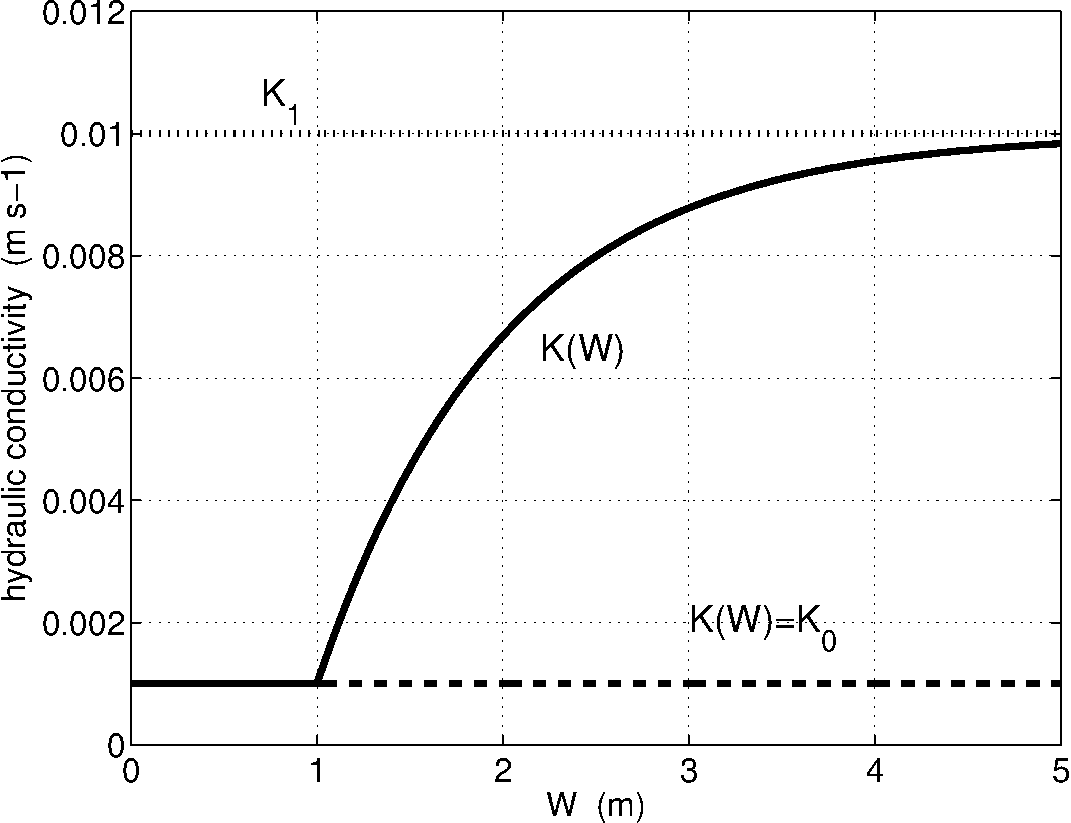
\includegraphics[width=3.5in,keepaspectratio=true]{figs/Kcompare}
\medskip
\caption{Function $K(W)$ defined by \eqref{eq:nontrivialK} (solid) has a bounded derivative but also has an abrupt change in behavior at $W=W_r$.  The constant case $K(W)=K_0$ is also shown (dashed).  Parameters $W_r=1,K_0=0.001,K_1=0.01$ are chosen for illustration.}
\label{fig:Kcompare}
\end{figure}

The mathematical model is now fully-specified:
\begin{empheq}[box=\mybluebox]{align}
0 &\le W, \notag \\
0 &\le P \le P_o, \notag \\
\psi &= P + \rho_w g (b + W), \notag \\
K(W) &= K_1 + (K_0-K_1) \exp\left((W-W_r)_+/W_r\right), \notag \\
\bV &= - \frac{K(W)\,W}{\rho_w g} \grad P - K(W) \grad b, \label{eq:bluebox} \\
\frac{E_0}{P_o} \frac{\partial P}{\partial t} &= \Div \left(\frac{K(W)\,W}{\rho_w g}\, \grad \psi \right) + c_2 A (P_o - P)^3 (W+Y_0) - c_1 |\bv_b| (W_r - W)_+ + \Phi, \notag \\
\frac{\partial W}{\partial t} + &\Div\left(\bV\, W\right) = \Div \left(K(W)\, W \grad W\right) + \Phi. \notag
\end{empheq}

Model equations \eqref{eq:bluebox} relate the three classes of symbols in Table \ref{tab:symbols}.  (Additional symbols $\psi$ and $\bV$ are derived from these.)  The state functions $W$ and $P$ evolve according to model \eqref{eq:bluebox}.  Only the state functions must be provided with initial values, and only they must be saved when stopping and restarting a time-dependent numerical model.  The scalar parameters are all constant (i.e.~time- and space-independent) in the current context, though they could be allowed to vary spatially if desired.  Default values must be chosen for these parameters, but exploration of the parameter space is appropriate.  The data functions are, in practice, supplied by an ice sheet model.  

\begin{table}[ht]
\caption{Symbols used in subglacial hydrology model \eqref{eq:bluebox}.}
\begin{tabular}{r|c}
class & symbols \\ \hline
\emph{state functions} & $W$, $P$ \\
\emph{scalar parameters} & $A$, $c_1$, $c_2$, $E_0$, $g$, $K_0$, $K_1$, $\rho_i$, $\rho_w$, $W_r$, $Y_0$ \\
\emph{data functions} & $b$, $\Phi$, $P_o$, $|\bv_b|$ \\
\hline
\end{tabular}
\label{tab:symbols}
\end{table}


\section{Steady states}  \label{sec:steadyverif}

\subsection*{Processes become decoupled in steady state}  In this section we address only the $K(W)=K_0$ case.  The steady states of mathematical model \eqref{eq:bluebox} are worth considering both because the physical subglacial system is close to steady state much of the time, and because in the steady state case we can more easily find an exact solution.

Recall that the flux has two expressions $\bq = - K_0 (\rho_w g)^{-1} W \grad \psi = \bV W - K W \grad W$.  Thus, here is a steady form of model \eqref{eq:bluebox} which is written in terms of $\bV,\bq,W,P$:
\begin{align}
\bV &= - \frac{K_0}{\rho_w g} \grad P - K_0 \grad b, \label{eq:Vsteady} \\
\bq &= \bV W - K_0 W \grad W, \label{eq:qsteady} \\
0 &= - \Div \bq + \Phi, \label{eq:masscontsteady} \\
0 &= c_2 A (P_o - P)^3 (W+Y_0) - c_1 |\bv_b| (W_r - W)_+. \label{eq:openclosesteady}
\end{align}
In the last equation we have eliminated ``$- \Div \bq + \Phi$'' because it is zero.  Note that we also have bounds $W\ge 0$ and $0 \le P \le P_o$.

\begin{table}[ht]
  \centering
  \caption{Physical constants and major model parameters used throughout the paper.}
  \begin{tabular}{lllp{3.0in}} 
    \textbf{Name} & \textbf{Value} & \textbf{Units} & \textbf{Description}\\
\hline
    $A$ & $3.1689\times 10^{-24}$ & $\text{Pa}^{-3}\,\text{s}^{-1}$ & ice softness \citep{EISMINT96} \phantom{$\Big|$} \\
    $c_1$ & $0.5$ & $\text{m}^{-1}$ & cavitation coefficient in \eqref{eq:capacity} \\
    $c_2$ & $0.04$ & & creep closure coefficient in \eqref{eq:capacity} \\
    $E_0$ & $1.0$ & m & regularization thickness in \eqref{eq:dampeddstrong} \\
    $g$ & $9.81$ & m $\text{s}^{-2}$ & acceleration of gravity \\
    $\rho_i$ & $910$ & $\text{kg}\,\text{m}^{-3}$ & ice density \citep{GreveBlatter2009} \\
    $\rho_w$ & $1000$ & $\text{kg}\,\text{m}^{-3}$ & fresh water density \citep{GreveBlatter2009} \\
    $W_r$ & $1$ & $\text{m}$ & roughness scale in \eqref{eq:capacity} \\
    $Y_0$ & $0.001$ & m & regularization for layer thickness in \eqref{eq:closingform} \\
    \hline
  \end{tabular}
 \label{tab:constants}
\end{table}

Relative to the time-dependent form \eqref{eq:bluebox}, processes have become decoupled in the steady state equations \eqref{eq:Vsteady}--\eqref{eq:openclosesteady}.  There are separate balances between the divergence of the flux and the water input on the one hand (i.e.~equation \eqref{eq:masscontsteady}), and the opening and closing processes on the other hand (i.e.~equation \eqref{eq:openclosesteady}).  Steady state equations \eqref{eq:Vsteady}--\eqref{eq:openclosesteady} are identical to those of the \cite{Schoofetal2012} model, where the same decoupling is also noted.  Specifically, in the one-dimensional case the above equations reduce to (5.8) and (5.10) from \cite{Schoofetal2012}.


\subsection*{Functional relationship for pressure in steady state}  Equation \eqref{eq:openclosesteady} allow us to write the pressure $P=P(W)$ in steady state as a continuous function of the water amount $W$.  This fact was already pointed out in considering the steady states of equation \eqref{eq:hewittcapacity}.  In particular, steady state is only possible if \eqref{eq:steadyOCbound} holds, but here with $W$ for $Y$:
\begin{equation}
c_1 |\bv_b| (W_r - W)_+ \le c_2 A P_o^3 (W+Y_0) \qquad \text{ in steady state}. \label{eq:steadyboundfirst}
\end{equation}
In this and later formulas define
\begin{equation}
s_b =  \left(\frac{c_1 |\bv_b|}{c_2 A}\right)^{1/3},  \label{eq:definesb}
\end{equation}
a scaled basal sliding speed which has units of pressure.  (One may think of $s_b$ as a scale for the pressure drop associated to cavitation in steady state.)  Then \eqref{eq:steadyboundfirst} is equivalent to
\begin{equation}
W \ge W_c := \frac{s_b^3 W_r - P_o^3 Y_0}{s_b^3 + P_o^3} \qquad \text{ in steady state}. \label{eq:steadyboundsecond}
\end{equation}
This condition says that the water amount is above a critical level that depends on the sliding and the overburden pressure.  Inequalities \eqref{eq:steadyboundfirst} and \eqref{eq:steadyboundsecond} are less restrictive in the regularized case $Y_0>0$ than in the unregularized case $Y_0=0$.

If \eqref{eq:steadyboundfirst} or \eqref{eq:steadyboundsecond} holds then
\begin{equation}
P(W) = P_o - s_b \left(\frac{(W_r - W)_+}{W+Y_0}\right)^{1/3} \qquad \text{ in steady state}.  \label{eq:PofWsteady}
\end{equation}
Note that in \eqref{eq:PofWsteady} we have $P(W_c)=0$.  Underpressure ($P=0$) with subcritical water amount ($W<W_c$) does not occur in steady state though it can and does occur in nonsteady conditions.  

Formula \eqref{eq:PofWsteady} may apply even if $W\ge W_r$, in which case the water pressure takes the overburden value $P = P_o$.  However, if $P_o=0$ then \eqref{eq:steadyboundfirst} implies that either $W\ge W_r$ or $|\bv_b|=0$.  This describes the values of $W$ and $|\bv_b|$ at ice margins where $H\to 0$ and therefore $P_o\to 0$.

The rest of this section uses the specific values in Table \ref{tab:constants}.

\newcommand{\upto}{ \!\!\nearrow\! }
\newcommand{\downto}{ \!\searrow\! }
Figure \ref{fig:psteady-vb} shows the function $P(W)$ from \eqref{eq:PofWsteady} for several cases of uniform sliding speed $|\bv_b|$.  Figure \ref{fig:psteady-Po} shows $P(W)$ for several cases of uniform overburden pressure $P_o$.  Replacing $Y_0=0$ makes no apparent difference in these figures; not shown.  We see that as the water amount reaches the roughness scale ($W\upto W_r$) the pressure rises rapidly to overburden ($P(W) \upto P_o$).  At the other extreme, we see that $P(W) \downto 0$ if $W \downto W_c$.  The curves $P(W)$ in Figures \ref{fig:psteady-vb} and \ref{fig:psteady-Po}, which describe steady state, do not include the interval $0\le W < W_c$ because such underpressure conditions are not achievable in steady state.

\begin{figure}[ht]
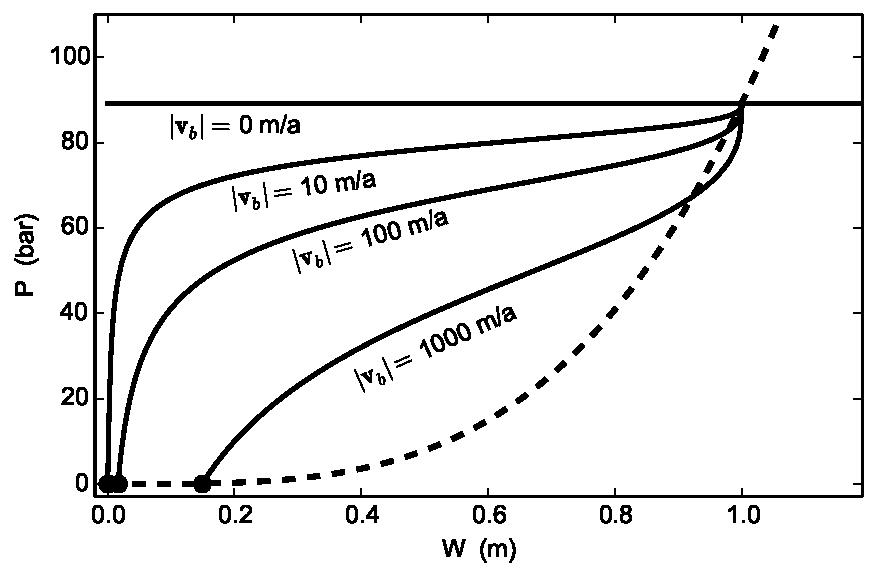
\includegraphics[width=3.5in,keepaspectratio=true]{figs/psteady-vb}
\medskip
\caption{The steady state function $P(W)$ defined by equation \eqref{eq:PofWsteady} depends on the sliding speed.  Four cases are shown (in color) using a fixed uniform ice thickness of $H=1000$ m: $|\bv_b|=0$ m/a (blue), $10$ m/a (green), $100$ m/a (red), and $1000$ m/a (cyan).  The values of $W_c$ for these cases are indicated by black dots with $P(W_c)=0$.  Relations \eqref{eq:PofWFC} (dashed black) and \eqref{eq:PofWBB} (dash-dot black) are shown with $W_{\text{crit}}=W_r$ for comparison.}
\label{fig:psteady-vb}
\end{figure}

\begin{figure}[ht]
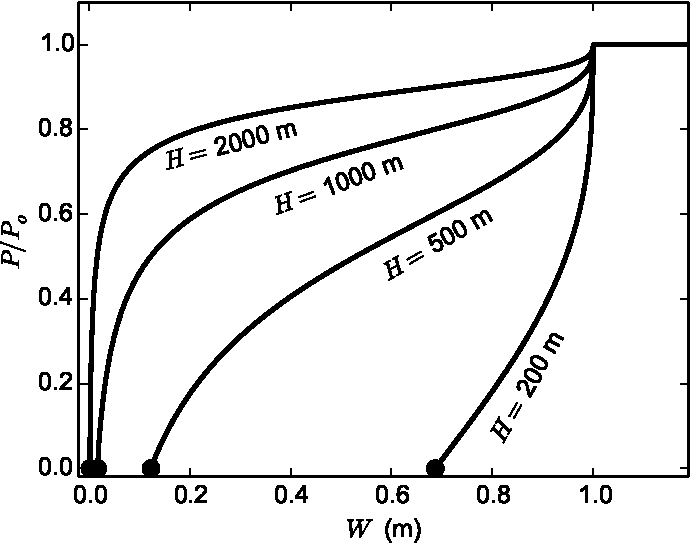
\includegraphics[width=3.5in,keepaspectratio=true]{figs/psteady-Po}
\medskip
\caption{Function $P(W)$ defined by \eqref{eq:PofWsteady} also depends on overburden pressure $P_o=\rho_i g H$.  We fix $|\bv_b|=100$ m/a and consider four cases of uniform thickness $H=$ $2000$ m (blue), $1000$ m (green), $500$ m (red), and $200$ m (cyan).}
\label{fig:psteady-Po}
\end{figure}

Recall that \cite{FlowersClarke2002_theory} propose the functional relation \eqref{eq:PofWFC} for both steady and nonsteady circumstances.  On the one hand formula \eqref{eq:PofWFC} has features in common with equation \eqref{eq:PofWsteady}: both functions $P(W)$ and $P_{FC}(W)$ are increasing and both relate the water pressure to the overburden pressure $P_o$.  However, while in \eqref{eq:PofWsteady} the relation to $P_o$ is additive, in \eqref{eq:PofWFC} it is a multiplicative scaling.  The power law form \eqref{eq:PofWFC} is not justified by the physical reasoning which led to equation \eqref{eq:PofWsteady}, even in steady state.   It would appear that any functional relationship $P(W)$ should also depend on the sliding velocity if cavitation is an influence on the water pressure.  For example, in the small sliding cases (e.g.~$|\bv_b| \ll 10$ m/a) creep will force $P(W) \approx P_o$ for a modest amount of water ($W\ll W_r$).  Of course the $W>W_{\text{crit}}$ case gives $P_{FC}(W) > P_o$ in \eqref{eq:PofWFC}, a problematic condition already noted by \cite{Schoofetal2012}.  This condition $P>P_o$ does not arise in \eqref{eq:PofWsteady} nor in the \cite{Schoofetal2012} theory.  Perhaps the most important contrast between the \cite{FlowersClarke2002_theory} theory and the current paper is that we have no functional relationship $P=P(W)$ in nonsteady conditions.

\subsection*{Velocity in steady state}  We now consider how the steady state water velocity $\bV$ depends on other quantities.  Equation \eqref{eq:PofWsteady} defines $P=P(W,P_o,s_b)$ while $\bV$ depends on $\grad P$, and thus we need derivatives of $P$.  In particular, in steady state we have
\begin{equation}
\frac{\partial P}{\partial W} =
    \begin{cases}
      \text{undefined}, & W \le W_c, \\
      \frac{1}{3} s_b (W_r + Y_0) (W+Y_0)^{-4/3} (W_r - W)^{-2/3}, & W_c < W < W_r, \\
      \text{undefined}, & W = W_r, \\
      0, & W > W_r.
    \end{cases}  \label{eq:dPdWsteady}
\end{equation}
Figures \ref{fig:psteady-vb} and \ref{fig:psteady-Po} illustrate these cases.  Note that the condition $W_c < W < W_r$ is identical to the normal pressure condition $0 < P < P_o$ in steady state.  Formula \eqref{eq:dPdWsteady} and the Figures agree that $\partial P / \partial W \to \infty$ as $W \upto W_r$.  Equations \eqref{eq:Vsteady}, \eqref{eq:PofWsteady}, and \eqref{eq:dPdWsteady} yield this formula for the velocity in steady state which applies in the normal pressure cases:
\begin{align}
\bV &= - \frac{K_0}{\rho_w g} \grad P - K_0 \grad b = - \frac{K_0}{\rho_w g} \left[\frac{\partial P}{\partial P_o} \grad P_o + \frac{\partial P}{\partial s_b} \grad s_b + \frac{\partial P}{\partial W} \grad W\right] - K_0 \grad b  \notag \\
    &= - \frac{K_0}{\rho_w g} \left[\grad \psi_o - \left(\frac{W_r - W}{W+Y_0}\right)^{1/3} \grad s_b + \frac{s_b (W_r + Y_0)}{3  (W+Y_0)^{4/3} (W_r - W)^{2/3}} \grad W\right]. \label{eq:Vsteadyexpand}
\end{align}
We have simplified the last expression by combining terms using the purely-geometrical function $\psi_o = P_o + \rho_w g b = \rho_i g H + \rho_w g b$ which we call the \emph{overburden potential}.  It is the hydraulic potential associated to an infinitesimal amount of water in the subglacial layer if it is at zero effective pressure.

Equation \eqref{eq:Vsteadyexpand} can help us understand the advective flux $\bV W$ part of $\bq=\bV W - K_0 W \grad W$.  First, the direction of water transport $\bV$ is determined in steady state by a combination of a geometric direction ($\grad \psi_o$), a direction derived from variations in the sliding speed ($\grad s_b$), and a diffusive direction.  The last category includes all terms proportional to $-\grad W$, thus both the known diffusive flux $-K_0 W \grad W$ and also the third term in \eqref{eq:Vsteadyexpand}.

We see that in steady state we have
\begin{equation}
\bq = - \alpha(W) \grad \psi_0 - \beta(W) \grad s_b - \gamma(W,s_b) \grad W  \label{eq:qabstract}
\end{equation}
for some coefficients $\alpha,\beta,\gamma$ which we now consider.  Restricting to the $Y_0=0$ case for simplicity, the first two coefficients $\alpha(W)$ and $\beta(W)$ go to zero as $W\to 0$.  However $\gamma(W,s_b)$ remains large when $W\to 0$, even if $K$ is small, as long as sliding is sustained ($s_b > 0$).  Thus for low water amount we should think of the water as diffusing in the layer \citep[compare equation (11) in][]{BBssasliding}.  When the water thickness closely approximates the roughness scale ($W\approx W_r$) then the second sliding term (i.e.~proportional to $\grad s_b$) contributes little while the third diffusive term is again strong if there is significant sliding.

Thinking more generally, it is no surprise that when the ice thickness, bed elevation, sliding velocity, or water thickness are highly variable in space then we can expect a larger amount of flow, and formula \eqref{eq:Vsteadyexpand} illustrates this.  Because the magnitude of the velocity $|\bV|$ determines the CFL time step restriction \citep{MortonMayers} associated to numerically solving the mass conservation equation in the model \eqref{eq:bluebox}, large variations in the same fields will generally reduce the time steps taken by a numerical model.


\subsection*{The radial case}  The above steady equations will be the basis for building a useful two-dimensional nearly-exact solution for $W$ and $P$.  This solution will depend on a single numerical solution of a first-order ODE which can be solved to very high precision.  Exact solutions in one horizontal dimension appear in \cite{Schoofetal2012}.  Here, by contrast, we consider a two horizontal dimension ice sheet geometry on a flat bedrock but our solution will only depend on the radial coordinate $r = \sqrt{x^2+y^2}$.  We derive the ODE now, after which we proceed to specify a particular exact solution for our verification purpose.

Consider steady state equations \eqref{eq:Vsteady}--\eqref{eq:masscontsteady} and eliminate $\bV$.  In the flat bed case the resulting pair of equations is
\begin{align}
q &= - \frac{K_0}{\rho_w g} W\, \left(\frac{dP}{dr} + \rho_w g \frac{dW}{dr}\right), \label{eq:rsflux} \\
\frac{1}{r}\frac{d}{dr}\left(r\,q\right) &= \Phi. \label{eq:rsconserve}
\end{align}
In the case of constant water input $\Phi(r)=\Phi_0$, which we assume for the exact solution, from \eqref{eq:rsconserve} we can integrate from $0$ to $r$ and use symmetry ($q(0)=0$) to get
\begin{equation}
q(r) = \frac{1}{2} \Phi_0\, r. \label{eq:qradial}
\end{equation}

On the other hand, equation \eqref{eq:PofWsteady} gives $P$ as a function of $W$ in steady state.  Suppose $h(r)$ is given so that $P_o(r)$ is also determined.  Assume that the scaled sliding speed $s_b(r)$ has a bounded derivative and that the solution $W(r)$ satisfies the normal pressure conditions $W_c < W < W_r$; both of these properties must be verified later for the constructed solution.  Now, by combining \eqref{eq:rsflux}, \eqref{eq:qradial}, \eqref{eq:PofWsteady}, and \eqref{eq:dPdWsteady} we can eliminate $q$ and $P$ to find
\begin{equation}
\varphi_0\, r = - W\, \left(\frac{dP_o}{dr} - \frac{ds_b}{dr} \left(\frac{W_r - W}{W+Y_0}\right)^{1/3} + \left(\frac{s_b (W_r + Y_0)}{3 (W+Y_0)^{4/3} (W_r - W)^{2/3}} + \rho_w g\right) \frac{dW}{dr}\right)  \label{eq:ODEfirst}
\end{equation}
in cases where $W_c < W < W_r$ and where $\varphi_0 = \rho_w g \Phi_0 (2 K_0)^{-1}$. 

Equation \eqref{eq:ODEfirst} is a first-order ordinary differential equation (ODE) for $W(r)$.  To put it in the standard form expected by a numerical ODE solver, solve for $dW/dr$:
\begin{equation}
\frac{dW}{dr} = \frac{\frac{ds_b}{dr} (W+Y_0) (W_r - W) - \Big[\varphi_0\, r W^{-1} + \frac{dP_o}{dr}\Big] (W + Y_0)^{4/3} \left(W_r - W\right)^{2/3}}{\frac{1}{3} s_b (W_r + Y_0) + \rho_w g (W + Y_0)^{4/3} (W_r - W)^{2/3}}.
\label{eq:WradialODE}
\end{equation}
Note that ODE \eqref{eq:WradialODE} has a constant solution $W(r)=W_r$.  To determine a nontrivial nearly-exact solution of this ODE we must choose an ice thickness $H(r)$ and a sliding speed $|\bv_b|(r)$ to determine $dP_o/dr$ and $ds_b/dr$, respectively.  The numerical solution of ODE \eqref{eq:WradialODE} will proceed from the ice margin at $r=L$ inward toward the center.


\section{A nearly-exact steady solution}

To generate a nontrivial exact solution we will have a positive thickness of ice at the margin so that $P_o(L^-)>0$.  Thus Figure \ref{fig:Pexact} shows a small cliff at the margin in the exact solution generated in this section.  We also assume that at the margin there is some sliding so that $s_b(L^-)>0$, and indeed we require that $s_b(L^-) W_r > P_o(L^-)^3 Y_0$.  At the ice margin $r=L$ we have water pressure $P=0$ so $W(L)=W_c(L^-)$ is the boundary (initial) condition for the ODE.  The initial condition at $r=L$ also satisfies $W(L) < W_r$.  Then we integrate \eqref{eq:WradialODE} from $r=L$ to $r=0$, and the central value $W(0)$ is determined as part of the solution.

\subsection*{Chosen surface elevation and sliding velocity}  It is useful to have an ice cap geometry $h(r)$ in which the surface gradient formula is simple so that $dP_o/dr$ in \eqref{eq:WradialODE} is also simple.  The plug flow, flat bed surface elevation solution of \cite{Bodvardsson} has this property.  Extending to the radial case, equations (23) and (24) of \citep{Bodvardsson} give
\begin{equation}
h(r) = h_0 \left(1 - \frac{r^2}{R_0^2} \right) \label{eq:choosebodvardssonh}
\end{equation}
where $h(0)=h_0$ is the height of the center of the ice cap.  It follows that $dP_o/dr = - C r$ where $C=2\rho_i g h_0 R_0^{-2}$.  We choose $L=0.9 R_0$ and we note that $h(L)=0.19 h_0$ in \eqref{eq:choosebodvardssonh}.

The sliding speed could be determined by a model for stresses at the ice base and within the ice \citep{GreveBlatter2009}, but a coupled ice and water dynamics solution is too advanced for the current purpose of primary hydrology model verification.  Instead we choose a well-behaved sliding speed function which has no sliding near the ice cap center, and which increases in the radial direction:
\begin{equation}
|\bv_b|(r) = \begin{cases} 0, & 0 \le r \le R_1, \\
                           v_0  \left(\frac{r-R_1}{L-R_1}\right)^5, & R_1 < r \le L.
             \end{cases}  \label{eq:choosevb}
\end{equation}
It follows from \eqref{eq:definesb} and \eqref{eq:choosevb} that $ds_b/dr$ in \eqref{eq:WradialODE} is bounded and continuous on $0\le r \le L$.

\subsection*{Numerical solution of radial ODE to give nearly-exact $W(r)$}  Now we can solve ODE \eqref{eq:WradialODE} with initial condition $W(L)=W_c(L)$ and the specific values in Table \ref{tab:verifconstants} by using an adaptive numerical ODE solver.  The result $W(r)$ is shown in Figure \ref{fig:Wexact}.  Equations \eqref{eq:choosebodvardssonh} and \eqref{eq:choosevb} also imply a pressure functional relation $P=P(W,r)$ from \eqref{eq:PofWsteady}.  This relation allows us to also show in Figure \ref{fig:Wexact} the regions of the $r,W$ plane which correspond to overpressure, normal pressure, and underpressure (solid curves).  We see that $W(r)$ is in the normal pressure region as $r$ decreases from $r=L$ to $r=R_1$.  At $r=R_1$ the function $W(r)$ switches into the overpressure case because there is no sliding.

\begin{table}[ht]
  \centering
  \caption{Constants used in constructing the nearly-exact solution.}
  \begin{tabular}{lllp{3.0in}}
    \textbf{Name} & \textbf{Value} & \textbf{Units} & \textbf{Description}\\
\hline
    $\Phi_0$ & $20$ & $\text{cm}\,\text{a}^{-1}$ & water input rate \\
    $h_0$ & $500$ & m & ice cap center thickness \\
    $K_0$ & $0.01$ & $\text{m}\,\text{s}^{-1}$ & constant hydraulic conductivity \\
    $L$   & $22.5$& km & $=0.9 R_0$; actual ice cap margin \\
    $R_0$ & $25$  & km & ideal ice cap radius \\
    $R_1$ & $5$   & km & radial location $r=R_1$ of onset of sliding \\
    $v_0$ & $100$ & $\text{m}\,\text{a}^{-1}$ & sliding speed scale \\
    \hline
  \end{tabular}
 \label{tab:verifconstants}
\end{table}

\begin{figure}[ht]
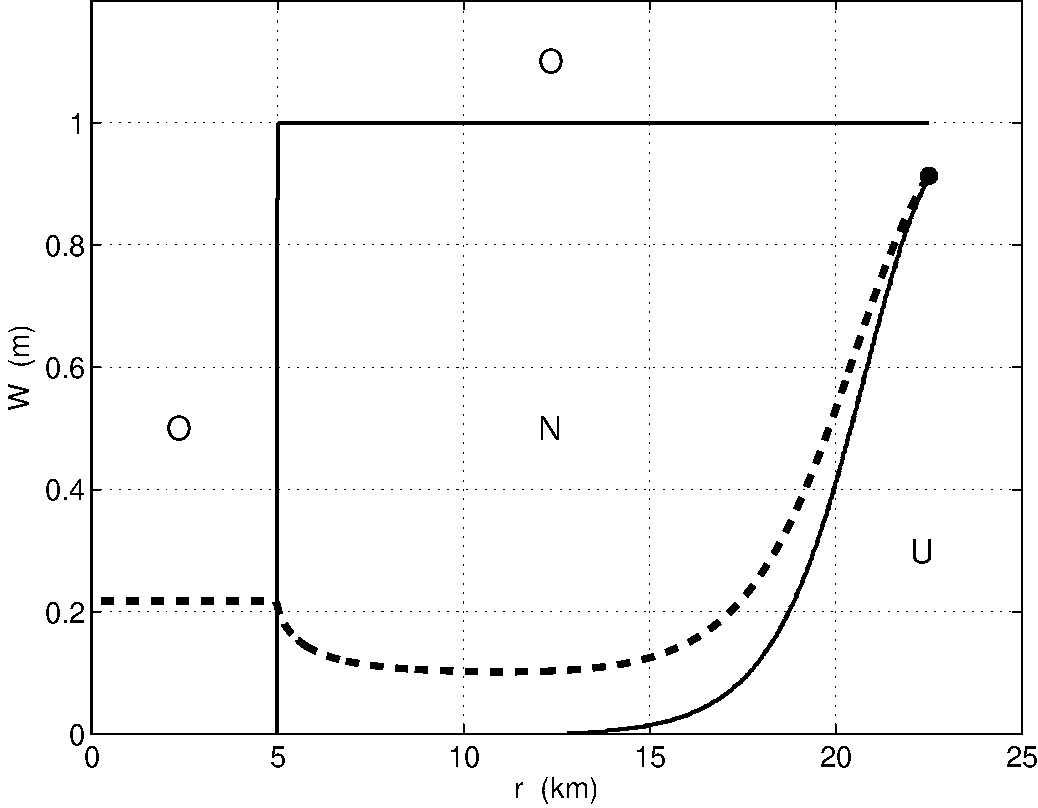
\includegraphics[width=3.5in,keepaspectratio=true]{figs/exact-W-plot-onu}
\caption{Nearly-exact radial, steady solution for water thickness $W(r)$ (dashed).  In $r$-versus-$W$ space the overpressure (O), normal pressure (N), and underpressure (U) regions are determined by ice geometry and sliding velocity (solid curves; see text).}
\label{fig:Wexact}
\end{figure}

To generate $W(r)$ in Figure \ref{fig:Wexact} we used both the standard, non-stiff Runge-Kutta 4(5) Dormand-Prince method, which is \Matlab's \texttt{ode45}, and the stiff, variable-order solver \texttt{ode15s}, with relative tolerance $10^{-12}$ and absolute tolerance $10^{-9}$, and with essentially identical results.
% could cite Shampine,Gladwell,Thompson (2003) on Matlab ODE solvers
Modest stiffness \citep{AscherPetzold} of ODE \eqref{eq:WradialODE} is observed for $r\approx R_1$, however.  The reason is that as the sliding goes to zero, the cavitation also goes to zero ($|\bv_b|\to 0$).  Because creep closure balances cavitation in steady state, it also goes to zero ($P\to P_o$).  The remaining active mechanisms in the model are variation in overburden pressure and the rate of water input.  They must exactly balance according to the steady mass conservation equation \eqref{eq:masscontsteady}.  In this case with no sliding ($s_b=0$), ODE \eqref{eq:WradialODE} reduces to the much simpler form
\begin{equation}
\frac{dW}{dr} = - \frac{\varphi_o r W^{-1} + \frac{dP_o}{dr}}{\rho_w g}. \label{eq:WradialODEnoslide}
\end{equation}
Equation \eqref{eq:WradialODEnoslide} is actually the steady radial form of the mass conservation equation under the ``$P=P_o$'' closure, namely equation \eqref{eq:PisoverConservation}.

In equation \eqref{eq:WradialODEnoslide} we see that $dW/dr=0$ if $W$ satisfies $W = - \varphi_0 r / (dP_o/dr)$.  In our case with geometry \eqref{eq:choosebodvardssonh} this reduces to a constant value $W=\tilde W= 0.21764$ m because $\Phi_0$ is constant and $dP_o/dr$ is linear in $r$.  Both numerical ODE solvers mentioned above confirm that $W(r)$ is asymptotic to this constant value $\tilde W$ as $r\to 0$, and that $W(r)\approx \tilde W$ within about 1\% on all of $0\le r \le R_1$.  This is seen in Figure \ref{fig:Wexact}.

\begin{figure}[ht]
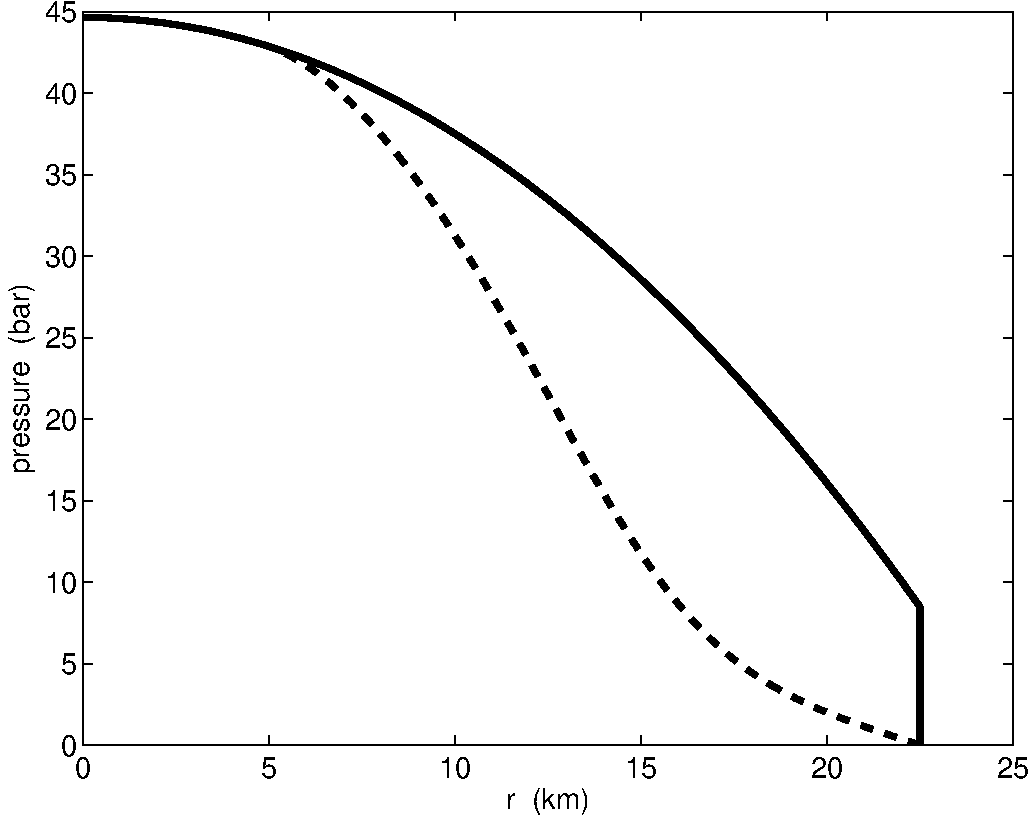
\includegraphics[width=3.5in,keepaspectratio=true]{figs/exact-P-plot}
\caption{Nearly-exact radial, steady solution pressure $P(r)$ (dashed) and overburden pressure $P_o$ (solid).}
% FIXME:  add second axis for velocity
\label{fig:Pexact}
\end{figure}


\section{Numerical schemes}  \label{sec:num}

\subsection*{Discretization of the mass conservation equation}  The mass conservation equation \eqref{eq:adeqn} will be discretized by an explicit, conservative finite difference method.   A centered, second-order scheme will be applied to the nonlinear diffusion part.  A pair of schemes for the advection part will be compared, first-order upwinding and a higher-order flux-limited upwind-biased method.

We first consider stable time steps.  The time step restriction for the advective part, namely the CFL condition for either of the schemes under consideration, is much more restrictive in this case than the time-step restriction for the diffusion.  Stability for these schemes occurs with a time step $\Delta t \le \Delta t_{\text{CFL}}$ where
\begin{equation}
\Delta t_{\text{CFL}} \left(\frac{\max |\alpha|}{\Delta x} + \frac{\max |\beta|}{\Delta y}\right) = \frac{1}{2}. \label{eq:dtCFL}
\end{equation}
Here $\bV=(\alpha,\beta)$ is the advection velocity.  The Appendix shows that this condition is sufficient for the first-order upwind scheme, but standard theory suggests the higher-order advection scheme has the same restriction \citep{HundsdorferVerwer2010}.  Because of the additional diffusion process, the time step should also satisfy $\Delta t \le \Delta t_{W}$ \citep{MortonMayers} where
\begin{equation}
\Delta t_W\, 2 \max(K(W) W) \left(\frac{1}{\Delta x^2} + \frac{1}{\Delta y^2}\right) = \frac{1}{2}. \label{eq:dtDIFFW}
\end{equation}
The condition $\Delta t \le \min\{\Delta t_{\text{CFL}}, \Delta t_W\}$ is a sufficient condition for stability and convergence of the overall scheme for \eqref{eq:adeqn}.

To understand these restrictions quantitatively, we consider typical values of the parameters.  The maximum water speed $|\bV|$ is about $10^5$ m/a in trial runs of the model, so $\max |\alpha| = \max |\beta| \approx 0.002$ m/s.  We take $K(W)=K_0=10^{-2}$ m/s from Table \ref{tab:verifconstants} and $\max W=1$ m as representative values.  Then, for a $\Delta x = \Delta y = 500$ m grid, the advective restriction \eqref{eq:dtCFL} is $\Delta t_{\text{CFL}} \approx 0.001$ year while the diffusive restriction from \eqref{eq:dtDIFFW} is $\Delta t_W \approx 0.1$ year.  Thus, unless velocities are unusually slow, or unless deep subglacial lakes develop so that $KW$ is large and $\Delta t_W$ is correspondingly small, we should not worry so much about this diffusive time scale.  There is significant uncertainty in these estimated values because the velocity field is a solution to the model.  The time step restrictions are applied adaptively, however, so stability is assured even though the total computational time is uncertain.

\begin{figure}[ht]
\centering
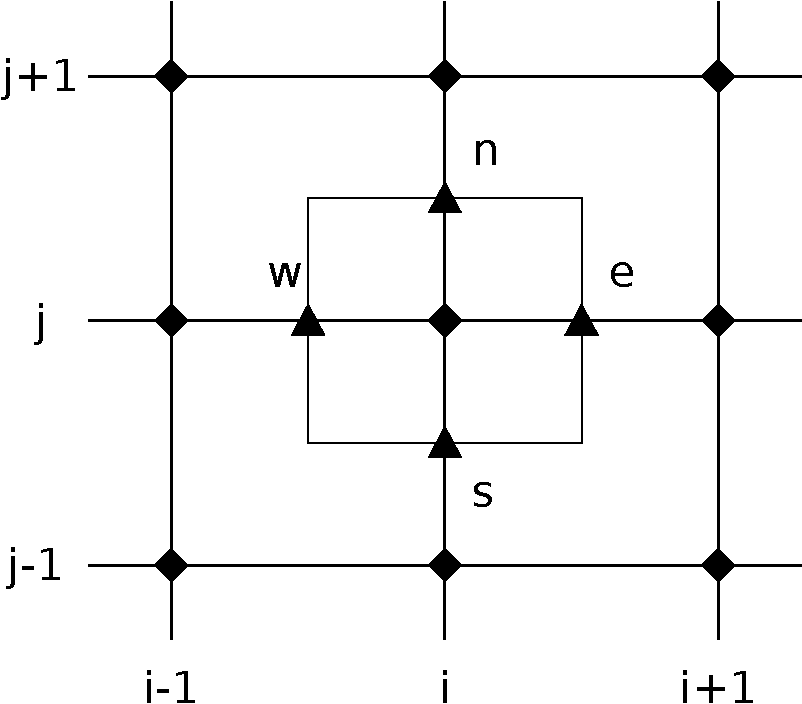
\includegraphics[width=2.9in,keepaspectratio=true]{figs/diffstencil}
\bigskip
\caption{Numerical scheme \eqref{eq:Wfd} for Equation \eqref{eq:adeqn} uses a grid-centered cell (dashed line).  The velocities, diffusivities, and fluxes are evaluated at the staggered grid locations (triangles) which are denoted with compass direction ($e,w,n,s$).  Scheme \eqref{eq:Pfd} has the same stencil.  The state functions $W,P$ live at the regular grid points (diamonds).}
\label{fig:stencil}
\end{figure}

To set notation, suppose our rectangular computational domain has $M_x \times M_y$ gridpoints $(x_i,y_j)$ with uniform spacing $\Delta x,\Delta y$.  Let $\Wlij \approx W(t_l,x_i,y_j)$ and $\Plij \approx P(t_l,x_i,y_j)$ be the approximations of the continuum solution at the grid points.  Recall that $\bV$ is determined from pressure and bed elevation by a formula in \eqref{eq:bluebox}.  Let $\bQ=\bV W$ so that $\Div \bQ = (\alpha W)_x + (\beta W)_y$.  We will compute velocity components and flux components at the staggered (cell-face-centered) points shown in Figure \ref{fig:stencil}.  We compute these values based on centered finite difference approximations of Equation \eqref{eq:vexpression}.

We use ``compass'' notation such as $\alpha_e = \alpha_{i+1/2,j}$ for the ``east'' staggered component.  Also when defining the velocity and the diffusive term (below) we will need staggered grid values of the water layer thickness, and again we use compass notation for these.  They are computed by averaging regular grid values:
\begin{equation}
W_e = (W_{i,j}^l + W_{i+1,j}^l)/2, \qquad W_n = (W_{i,j}^l + W_{i,j+1}^l)/2. \label{eq:stagW}
\end{equation}
In this case we can compute the ``west'' and ``south'' values by shifting our base point by one space: $W_w = W_e\big|_{(i-1,j)}$ and $W_s = W_n\big|_{(i,j-1)}$.

Now we can get the velocity components needed at staggered locations:
\begin{align}
\alpha_e &= - \frac{K(W_e)}{\rho_w g} \frac{P_{i+1,j}-P_{i,j}}{\Delta x} - K(W_e) \frac{b_{i+1,j}-b_{i,j}}{\Delta x}, \label{eq:velocitycomp} \\
\beta_n  &= - \frac{K(W_n)}{\rho_w g} \frac{P_{i,j+1}-P_{i,j}}{\Delta y} - K(W_n) \frac{b_{i,j+1}-b_{i,j}}{\Delta y}. \notag
\end{align}
Again $\alpha_w = \alpha_e\big|_{(i-1,j)}$ and $\beta_s = \beta_n\big|_{(i,j-1)}$; there are only two distinct staggered grid values (i.e.~$\alpha_e,\beta_n$) to compute per regular grid location $(x_i,y_j)$.

The face-centered (staggered-grid) normal fluxes $Q_e(\alpha_e)$, $Q_w(\alpha_w)$, $Q_n(\beta_n)$, and $Q_s(\beta_s)$ are components of the advective flux $\bV W$.  These quantities are described in more detail in the next subsection.  They use only the co-located (staggered) velocity component but there is upwinding to determine which $W$ value(s) are used.

Now we can state our scheme for equation \eqref{eq:adeqn}:
\begin{align}
 &\frac{W_{i,j}^{l+1} - \Wlij}{\Delta t} + \frac{Q_e(\alpha_e) - Q_w(\alpha_w)}{\Delta x} + \frac{Q_n(\beta_n) - Q_s(\beta_s)}{\Delta y}  \label{eq:Wfd} \\
      &\qquad = \frac{K(W_e) W_e \left(W_{i+1,j}^l - \Wlij\right) - K(W_w) W_w \left(\Wlij - W_{i-1,j}^l\right)}{\Delta x^2}  \notag \\
      &\qquad\qquad\qquad + \frac{K(W_n) W_n \left(W_{i,j+1}^l - \Wlij\right) - K(W_s) W_s \left(\Wlij - W_{i,j-1}^l\right)}{\Delta y^2} + \Phi_{ij}. \notag
\end{align}
Assuming no error in the flux components $Q$, the local truncation error \citep{MortonMayers} of scheme \eqref{eq:Wfd} would be $O(\Delta t^1 + \Delta x^2 + \Delta y^2)$.  The actual truncation error depends on the nature of the discrete fluxes, which we address next.


\subsection*{Flux discretization}  Because \eqref{eq:adeqn} is an advection-dominated PDE, the well-known goals for discretizing the fluxes include non-oscillation and positivity \citep{HundsdorferVerwer2010} in addition to reduced truncation error.  Schemes addressing these goals, which are often described as finite volume discretizations \citep{LeVeque}.  We now introduce a few such schemes using an advection-only model equation in which a quantity $u(t,x)$ is transported by a velocity $v(x)$:
\begin{equation} \label{eq:modeladvect}
u_t + (v(x) u)_x = 0
\end{equation}

Suppose that the grid points $x_i$ are the centers of equally-spaced cells with $x_{i+1}-x_i=\Delta x$.  Cell interfaces are at $x_{i-1/2}=x_w$ and $x_{i+1/2}=x_e$.  Suppose we do not discretize time and instead we denote $u_i=u_i(t)$.  We say a spatial discretization of \eqref{eq:modeladvect} is \emph{positive} if $u(0,x)\ge 0$ for all $x$ implies $u(t,x)\ge 0$ for all $t\ge 0$ and all $x$.  Clearly such a property is desirable for any conservation scheme for the water thickness $W$ because thicknesses are intrinsically nonnegative.

The basic discretization of \eqref{eq:modeladvect} uses the fluxes $Q=v(x) u$ at the cell interfaces $x_w$ and $x_e$, namely
\begin{equation}
\frac{du_i}{dt} + \frac{Q_e - Q_w}{\Delta x} = 0, \label{eq:basicmodelFD}
\end{equation}
but we must choose a flux parameterization.  The simplest positive scheme for the fluxes is first-order upwinding in conservative form \citep[section I.4.3]{HundsdorferVerwer2010}.  We use the upwind value $u_i$ for the flux at $x_e$ because $v_e = v(x_e) \ge 0$:
\begin{equation}
Q_e = v_e u_i \label{eq:upwindfluxfirst}
\end{equation}
Also $Q_w = v_w x_{i-1}$ because $v_w = v(x_w) \ge 0$.  Scheme \eqref{eq:upwindfluxfirst} is also called the ``donor cell'' upwind method \citep{LeVeque}.

A second-order truncation error scheme which is \emph{not} positive uses a centered average in computing the flux.  We can regard this as a correction to the first-order upwind form:
\begin{equation}
Q_e = v_e \frac{u_i+u_{i+1}}{2} = v_e \left[u_i + \frac{1}{2} (u_{i+1} - u_i)\right]. \label{eq:centerfluxfirst}
\end{equation}
A yet higher-resolution scheme is third-order upwind-biased fluxes which can again be written as a correction to first-order upwinding:
\begin{equation}
Q_e = v_e \frac{-u_{j-1} + 5 u_i + 2 u_{i+1}}{6} = v_e \left[u_i + \left(\frac{1}{3}+\frac{1}{6} \theta_i \right) (u_{i+1} - u_i)\right] \label{eq:thirdfluxfirst}
\end{equation}
where
\begin{equation}
\theta_i = \frac{u_{i} - u_{i-1}}{u_{i+1} - u_i}.  \label{eq:thetadefine}
\end{equation}
Unfortunately, despite the upwind-biasing in the third-order scheme, both \eqref{eq:centerfluxfirst} and \eqref{eq:thirdfluxfirst} cause oscillations and are not positive.

The approach of flux-limiting is to regard the corrections in \eqref{eq:centerfluxfirst} and \eqref{eq:thirdfluxfirst} as too large in some situations, for instance near local extrema of $u$, to allow positivity \citep[section III.1.1]{HundsdorferVerwer2010}.  Unfortunately, Godunov's barrier theorem \citep[section I.7.1]{HundsdorferVerwer2010} says that we cannot get truncation error better than first-order with a discretization that is both linear and positive.  On the other hand there exist nonlinear ``flux-limited'' (correction-limited) formulas which restore these properties.  Because the schemes under consideration are explicit, the nonlinearity itself does not represent a significant computational cost.

These flux-limited schemes can be written in the same general form as above, with a correction to the first-order upwinded flux:
\begin{equation}
Q_e = v_e \left[u_i + \psi(\theta_i) (u_{i+1} - u_i)\right], \qquad v_e \ge 0. \label{eq:fluxlimiterform}
\end{equation}
If we have $v(x)<0$ in \eqref{eq:modeladvect} then the same function $\psi$ should be used but with the direction reversed \citep[section III.1.1]{HundsdorferVerwer2010}:
\begin{equation}
Q_e = v_e \left[u_{i+1} + \psi\left((\theta_{i+1})^{-1}\right) (u_i - u_{i+1})\right], \qquad v_e < 0. \label{eq:fluxlimiterformreversed}
\end{equation}
The forms for $Q_w$ in \eqref{eq:basicmodelFD} simply replace $v_e \to v_w$, $i\to i-1$, and $i+1\to i$.  Table \ref{tab:fluxlimiters} shows several cases for $\psi$ including those already considered.

The difference ratio $\theta_i$ in \eqref{eq:thetadefine} can take any real value.  For the time-discretizations we will consider, sufficient conditions on $\psi(\theta)$ to give a positive advection scheme for model equation \eqref{eq:modeladvect} are
\begin{equation}
0 \le \psi(\theta) \le 1, \qquad 0 \le \frac{\psi(\theta)}{\theta} \le 1 \qquad \text{ for all } \theta \in \RR.
\end{equation}
The schemes in Table \ref{tab:fluxlimiters} which satisfy these conditions are marked with ``$\ast$''.

For smooth functions and fine grids we have $\theta_i\approx 1$ except near extrema where $u_{i+1} - u_i$ and $u_i - u_{i-1}$ are both near zero.  Note that in every case in Table \ref{tab:fluxlimiters} where there is a correction ($\psi(\theta)\ne 0$) we have $\psi(1)=1/2$.  The Koren flux-limiter in Table \ref{tab:fluxlimiters}, which we will demonstrate in practice, has $\psi(\theta) = \frac{1}{3}+\frac{1}{6} \theta$ for $\frac{2}{5} \le \theta \le 4$.  Therefore we can think of the Koren scheme as a positive form of the third-order upwind-biased scheme.

\begin{table}[ht]
  \centering
  \caption{Flux schemes written in limiter form \eqref{eq:fluxlimiterform} using $\theta=\theta_i$ from \eqref{eq:thetadefine}.  See \cite{HundsdorferVerwer2010} for discussion of these and other schemes.}
  \begin{tabular}{ll}
    \textbf{scheme ($\ast=$ positive)} & \textbf{formula} \\
\hline
    $\ast$ first-order upwinding               & $\phantom{\Big|}\psi(\theta) = 0$ \\
    \phantom{$\ast$} second-order centered     & $\phantom{\Big|}\psi(\theta) = \frac{1}{2}$  \\
    \phantom{$\ast$} third-order upwind-biased & $\phantom{\Big|}\psi(\theta) = \frac{1}{3}+\frac{1}{6} \theta$  \\
    $\ast$ van Leer 1974                       & $\phantom{\Big|}\psi(\theta) = \frac{1}{2} \frac{\theta + |\theta|}{1+\theta}$  \\
    $\ast$ Koren 1993                          & $\phantom{\Big|}\psi(\theta) = \max\left\{0,\min\{1,\theta,\frac{1}{3}+\frac{1}{6} \theta\}\right\}$  \\
    \hline
  \end{tabular}
 \label{tab:fluxlimiters}
\end{table}

To summarize our understanding of flux discretizations for model equation \eqref{eq:modeladvect}, first-order upwinding \eqref{eq:upwindfluxfirst} gives positivity but only $O(\Delta x^1)$ truncation error while second-order centered differencing \eqref{eq:centerfluxfirst} and third-order upwind-biased differencing \eqref{eq:thirdfluxfirst} give better truncation error (i.e.~$O(\Delta x^2)$ and $O(\Delta x^3)$, respectively), but not positivity.  The flux-limited Koren and van Leer schemes in Table \ref{tab:fluxlimiters} give positivity and also better truncation error away from difficult areas (i.e.~near extrema and non-smooth areas where $\theta_j$ is not near one), but they revert to first-order in these difficult areas.

The above discussion was limited to the spatial discretization; we have applied ``method of lines'' only.  A time discretization is also required, and for this we simply choose forward Euler.  Using one of the positive spatial discretizations above, the resulting fully discrete system is positive if
\begin{equation}
\max_x \frac{|v(x)|\Delta t}{\Delta x} \le \frac{1}{2}, \label{eq:CFL}
\end{equation}
as proven in section III.1.1 of \cite{HundsdorferVerwer2010}.  Section III.1.3 of the same reference shows these positive schemes are also total variation diminishing (TVD) if the velocity is constant ($v(x)=v_0$).  We will identify condition \eqref{eq:CFL} as simply ``CFL'' even though it is more strict than the CFL condition that suffices for stability \citep{MortonMayers}.

At this point we can state the two alternatives which we will actually test as discrete flux schemes in equation \eqref{eq:Wfd}.  Recall that the velocity has components $\bV=(\alpha,\beta)$ which are evaluated at these staggered locations following \eqref{eq:velocitycomp}.  Also recall that the flux at the staggered grid location $(x_{i+1/2},y_j)$ is denoted ``$Q_e(\alpha_e)$'' and that the flux at $(x_i,y_{j+1/2})$ is denoted ``$Q_n(\beta_n)$.''  To ensure conservation we must have a single formula for $Q_{i+1/2,j}$ whether this flux is ``$Q_e$'' for $(x_i,y_j)$ or ``$Q_w$'' for $(x_{i+1},y_j)$; similar comments apply to ``$Q_n$'' versus ``$Q_s$''.  Thus we simply give formulas for $Q_e$ and $Q_n$:
\begin{align}
Q_e(\alpha_e) &= \begin{cases} \alpha_e \left[W_{i,j} + \psi(\theta_{i}) (W_{i+1,j} - W_{i,j})\right], & \alpha_e \ge 0, \\ \alpha_e \left[W_{i+1,j} + \psi\left((\theta_{i+1})^{-1}\right) (W_{i,j} - W_{i+1,j})\right], & \alpha_e < 0, \end{cases} \label{eq:adfluxes} \\
Q_n(\beta_n) &= \begin{cases} \beta_n \left[W_{i,j} + \psi(\theta_{j}) (W_{i,j+1} - W_{i,j})\right], & \beta_n \ge 0, \\ \beta_n \left[W_{i,j+1} + \psi\left((\theta_{j+1})^{-1}\right) (W_{i,j} - W_{i,j+1})\right], & \beta_n < 0. \end{cases} \notag
\end{align}
The flux-limiters which we will consider are the first-order upwind ($\psi(\theta)=0$) and Koren ($\psi(\theta) = \max\left\{0,\min\{1,\theta,\frac{1}{3}+\frac{1}{6} \theta\}\right\}$) cases in Table \ref{tab:fluxlimiters}.  The subscripted $\theta$ quotients are as follows:
\begin{align*}
\theta_i &= \frac{W_{i,j}-W_{i-1,j}}{W_{i+1,j} - W_{i,j}}, & (\theta_{i+1})^{-1} &= \frac{W_{i+2,j}-W_{i+1,j}}{W_{i+1,j} - W_{i,j}}, \\
\theta_j &= \frac{W_{i,j}-W_{i,j-1}}{W_{i,j+1} - W_{i,j}}, & (\theta_{j+1})^{-1} &= \frac{W_{i,j+2}-W_{i,j+1}}{W_{i,j+1} - W_{i,j}}.
\end{align*}
Clearly one does not need to compute these ``$\theta$s'' when using first-order upwind.

When using the Koren flux-limiter the stencil in Figure \ref{fig:stencil} is incomplete.  In particular the additional regular grid neighbors $W_{i+2,j}$, $W_{i-2,j}$, $W_{i,j+2}$, $W_{i,j-2}$ are each (potentially) involved in updating $W_{i,j}$.

For either the first-order or high-resolution flux schemes, and even if the combined advection-diffusion scheme is still structurally-positive as is proved in the Appendix for first-order upwind fluxes, if the water input $\Phi$ is negative then we must actively enforce the positivity of the water thickness $W$.  That is, positivity of the advection-diffusion scheme is a highly-desirable property but it does not ensure positivity of the solution if there is actual water removal ($\Phi < 0$).  Generally we must project (reset) $W$ to be nonnegative at the end of each time step.


\subsection*{A numerical scheme for the ``lakes'' model}  Recall equation \eqref{eq:PisoverConservation} which came from the mass conservation equation and the assumption that the subglacial water pressure was equal to the overburden pressure.  We call this the ``lakes'' model because its primary purpose in the literature has been in the identification of the locations of subglacial lakes in Antarctica.  It simply pushes water toward the minima of the hydraulic potential.  We now have a numerical scheme that suffices for this model, and the more complete model we seek only adds a new pressure equation to this ``lakes'' model.

To be a little more careful, consider the model consisting of advection-decomposition equations \eqref{eq:vexpression} and \eqref{eq:adeqn}.  Furthermore suppose $P=\lambda P_o$ with $0<\lambda\le 1$ so that the pressure is a fixed fraction of overburden.  Then this model has advection-diffusion form \eqref{eq:adeqn} and it is well-posed.  Taken literally, the model \eqref{eq:PisoverConservation} which appears in the literature generally predicts subglacial lakes of infinitesimal extent if the bed elevation is differentiable but not continuously-so (and infinite depth in steady state); it is not well-posed in that sense.  Here the addition of the term ``$\rho_w g W$'' to the hydraulic potential, as used in this paper, provides a diffusive term which implies finite lakes.

The numerical schemes above suffice for this continuum ``lakes'' model, and they are implemented in PISM.  The more complete model, whose numerical implementation is described next, is logically an extension of this ``lakes'' (sub)model in which the artificial closure $P=\lambda P_o$ is replaced by a physically-motivated closure based on cavity opening and closing processes.


\subsection*{Discretization of the pressure evolution equation}  The pressure evolution equation \eqref{eq:diffusionpressure} is a nonlinear diffusion with additional ``reaction'' terms associated to opening and closing.  Unlike solving \eqref{eq:adeqn} for $W$, when solving \eqref{eq:diffusionpressure} for $P$ there is no dominating advection term.  Therefore we discretize it using an explicit centered, second-order scheme.  Again, because this is an explicit scheme, we consider stable time steps immediately.

The time step restriction is comparable to \eqref{eq:dtDIFFW}, though the proof in the appendix does not suffice to \emph{prove} stability under this condition because of the additional reaction terms.  Noting that $P_o=\rho_i g H$, the time step must satisfy $\Delta t \le \Delta t_P$ where
\begin{equation}
\Delta t_P\, \left(\frac{2 \rho_i \max H \max(K(W) W)}{\rho_w E_0}\right) \left(\frac{1}{\Delta x^2} + \frac{1}{\Delta y^2}\right) = \frac{1}{2} \label{eq:dtDIFFP}
\end{equation}
The resulting time step $\Delta t_P$ is a fraction of $\Delta t_W$ from \eqref{eq:dtDIFFW}:
\begin{equation}
\Delta t_P = \frac{\rho_w E_0}{\rho_i \max H}\, \Delta t_W.  \label{eq:dtDIFFPfromW}
\end{equation}
In fact, with the estimates $\rho_w/\rho_i \approx 1$, $E_0\approx 1$ m, and $\max H \approx 1000$ m we have $\Delta t_P$ which is about 1000 times smaller than $\Delta t_W$.  With these values and others used earlier (i.e.~$\Delta x = \Delta y = 500$ m, $\max |\bV|=10^5$ m/a, $K_0=10^{-2}$ m/s and $\max W=1$ m) we get
\begin{align*}
  \Delta t_{\text{CFL}} &\approx 0.001  \text{ year} &&\text{ from \eqref{eq:dtCFL}}, \\
  \Delta t_W            &\approx 0.1    \text{ year} &&\text{ from \eqref{eq:dtDIFFW}}, \\
  \Delta t_P            &\approx 0.0001 \text{ year} &&\text{ from \eqref{eq:dtDIFFP} or \eqref{eq:dtDIFFPfromW}.}
\end{align*}
Thus the numerical scheme for pressure diffusion, given next, has the shortest time step.  This analysis says if is only about 10 times shorter than the CFL restriction for the advection, however.  Furthermore, the precise size of the stable time step $\Delta t_P$ scales inversely with the adjustable small thickness $E_0$.  By choosing $E_0$ larger or smaller we can make the time step restriction on $\Delta t_P$ less or more severe, respectively.

Now, the scheme we use for \eqref{eq:diffusionpressure} is similar to \eqref{eq:Wfd} for \eqref{eq:adeqn} but without a need for approximating advection:
\begin{align}
\frac{E_0}{(P_o)_{i,j}} \frac{P_{i,j}^{l+1} - \Plij}{\Delta t} &= \frac{1}{\rho_w g} \bigg[\frac{K(W_e)\,W_e \left(\psi_{i+1,j}^l - \psi_{i,j}^l\right) - K(W_w)\,W_w \left(\psi_{i,j}^l - \psi_{i-1,j}^l\right)}{\Delta x^2}  \label{eq:Pfd} \\
      &\qquad\qquad + \frac{K(W_n)\,W_n \left(\psi_{i,j+1}^l - \psi_{i,j}^l\right) - K(W_s)\,W_s \left(\psi_{i,j}^l - \psi_{i,j-1}^l\right)}{\Delta y^2}\bigg] \notag \\
      &\qquad + c_2 A \left(\rho_i g H_{i,j}- \Plij\right)^3 \Wlij - c_1 |\bv_b|_{i,j} \left(W_r - \Wlij\right)_+ + \Phi_{i,j}. \notag
\end{align}
For implementation it is useful to restate \eqref{eq:Pfd} in explicit update form.  First define
	$$\omega_x = \frac{\Delta t}{\rho_w g \Delta x^2}, \qquad \omega_y = \frac{\Delta t}{\rho_w g \Delta y^2}.$$
Also let
	$$\mathcal{O}_{ij} = c_1 |\bv_b|_{i,j} \left(W_r - \Wlij\right)_+, \qquad \mathcal{C}_{ij} = c_2 A \left(\rho_i g H_{i,j} - \Plij\right)^3 \Wlij$$
be the gridded values of the cavitation-opening and creep-closure rates.  Then scheme \eqref{eq:Pfd} is equivalent to this form:
\begin{align}
P_{i,j}^{l+1} &= \Plij +  \frac{(P_o)_{i,j}}{E_0} \bigg[\omega_x K(W_e) W_e \left(\psi_{i+1,j}^l - \psi_{i,j}^l\right) - \omega_x K(W_w) W_w \left(\psi_{i,j}^l - \psi_{i-1,j}^l\right) \label{eq:Pfdupdate} \\
      &\qquad\qquad\qquad\quad + \omega_y K(W_n) W_n \left(\psi_{i,j+1}^l - \psi_{i,j}^l\right) - \omega_y K(W_s) W_s \left(\psi_{i,j}^l - \psi_{i,j-1}^l\right) \notag \\
      &\qquad\qquad\qquad\quad + \Delta t\, \left(\mathcal{C}_{ij} - \mathcal{O}_{ij} + \Phi_{i,j}\right)\bigg]. \notag
\end{align}

\subsection*{One time step of the model}  Mathematical model \eqref{eq:bluebox} evolves $W$ and $P$.  One time step of the fully-discretized evolution is described as follows, in the case that the ice geometry and ice sliding speed are fixed so that $h_{i,j}$, $b_{i,j}$, $(P_o)_{i,j}$, and $|\bv_b|_{i,j}$ are all determined for the duration of the run.  The ice geometry may be quite general, with ice-free land and floating ice allowed.  In fact, the ice geometry determines boolean masks for grid cell state based on a sea level of elevation zero:
\begin{align*}
\text{\texttt{icefree}}_{i,j} &= (h_{i,j} > 0)\, \&\, (h_{i,j} = b_{i,j}), \\
\text{\texttt{float}}_{i,j}   &= (\rho_i (H_{\text{float}})_{i,j} < - \rho_{sw}\, b_{i,j}).
\end{align*}
Here $H_{\text{float}}=h_{i,j} / (1 - r)$ is the thickness of the ice if it is floating, $r=\rho_i / \rho_{sw}$, and we take a sea-water density $\rho_{sw}=1028.0$.  Note that $\text{\texttt{float}}_{i,j}$ is true in ice-free ocean.  The subglacial layer we are attempting to model exists only for grounded ice, that is, only if both \texttt{icefree} and \texttt{float} masks are false.  The other mask cases provide boundary conditions when they are neighbors to grounded ice cells.  Now one time step follows this algorithm:

\bigskip\medskip
\renewcommand{\labelenumi}{\emph{(\roman{enumi})}}
\begin{enumerate}
\item Start with values $\Wlij$, $\Plij$ which satisfy the bounds $W\ge 0$ and $0 \le P \le P_o$.
\item Compute the current values of the hydraulic potential, $\psi_{i,j}^l = \Plij + \rho_w g(b_{i,j} + \Wlij)$, but with $\psi_{i,j}^l=(P_o)_{i,j}$ where $\text{\texttt{float}}_{i,j}$.
\item Compute velocity components $\alpha_e$, $\beta_n$ at staggered grid locations from \eqref{eq:velocitycomp}.
\item Get $W$ values averaged onto the staggered grid from \eqref{eq:stagW}.
%FIXME: however, Wea and Wno should not average from outside the ice domain?
\item Get time step $\Delta t = \min\{\Delta t_{\text{CFL}}, \Delta t_W, \Delta t_P\}$ using criteria \eqref{eq:dtCFL}, \eqref{eq:dtDIFFW}, and \eqref{eq:dtDIFFPfromW}.
\item If $\text{\texttt{icefree}}_{i,j}$ set $P_{i,j}^{l+1}=0$.  If $\text{\texttt{float}}_{i,j}$ then set $P_{i,j}^{l+1} = (P_o)_{i,j}$; this is the pressure of sea water at the base of the ice.  Then use \eqref{eq:Pfdupdate} to compute preliminary values for $P_{i,j}^{l+1}$ at the remaining locations.  Don't compute the $x$-($y$-)direction divided difference of the flux when either $x$-($y$-)neighbor is \texttt{icefree} or \texttt{float}.
\item If $P_{i,j}^{l+1}$ does not satisfy bounds $0 \le P \le P_o$ then reset (project) into this range.
\item Using \eqref{eq:adfluxes} and a particular flux-limiter, or first-order upwinding without flux limiter, compute the advective fluxes $Q_e(\alpha_e)$ at all staggered-grid points $(i+1/2,j)$ and $Q_n(\beta_n)$ at all staggered-grid points $(i,j+1/2)$.  
\item If $\text{\texttt{icefree}}_{i,j}$ or $\text{\texttt{float}}_{i,j}$ then set $W_{i,j}^{l+1}=0$.  Otherwise use \eqref{eq:Wfd} to compute preliminary values for $W_{i,j}^{l+1}$.
\item If $W_{i,j}^{l+1}<0$ then reset (project) $W_{i,j}^{l+1}=0$; this action is needed only when $\Phi<0$ because the rest of the $W$-update method is positivity-preserving.
\item Update time $t_{l+1}=t_l+\Delta t$ and repeat at \emph{(i)}.
\end{enumerate}

\bigskip\medskip
Any useful mass accounting scheme will keep track of the projections in steps \emph{(ix)} and \emph{(x)}.  In particular, water which is lost at the margin where either the thickness goes to zero on land, or at locations where the ice becomes floating (i.e.~at the grounding line), indeed may be the modeling goal.  (Users may be seeking the subglacial hydrological discharge at margin locations or at grounding lines!)  There is, however, no expectation that the pressure update step \emph{(vi)} will preserve bounds $0\le P \le P_o$.  As pressure is not a conserved quantity, however, the projection step \emph{(vii)} requires no special accounting.



\section{Numerical results}  \label{sec:results}

\subsection*{Verification of the coupled model}  By using the coupled steady-state nearly-exact solution constructed in section \ref{sec:steadyverif} we can now verify the numerical schemes described in section \ref{sec:num}.  Verification refers to the process of actually measuring the errors made by the numerical scheme, especially as the numerical grid is refined.  In this case our exact solution is for the steady-state so we initialize our time-stepping numerical scheme with the exact steady solution and we measure the error relative to the steady exact values after some period of time integration of the numerical scheme in section \ref{sec:num} for the full, time-dependent model \eqref{eq:bluebox}.  That is, we measure the drift away from the exact steady solution generated by the time-dependent numerical model.  The magnitude of that drift depends on the spatial grid size.  The rate of convergence under grid refinement is determined by the quality of our spatial discretizations.

We use the constants in Table \ref{tab:verifconstants}.  The exact solution is shown in Figures \ref{fig:Wexact} and \ref{fig:Pexact}.  We do a one month run on grids with spacing decreasing by factors of two from $6$ km to $375$ m.  The results, generated from Matlab codes, are shown in Figures \ref{fig:refineW} and \ref{fig:refineP}.

\begin{figure}[ht]
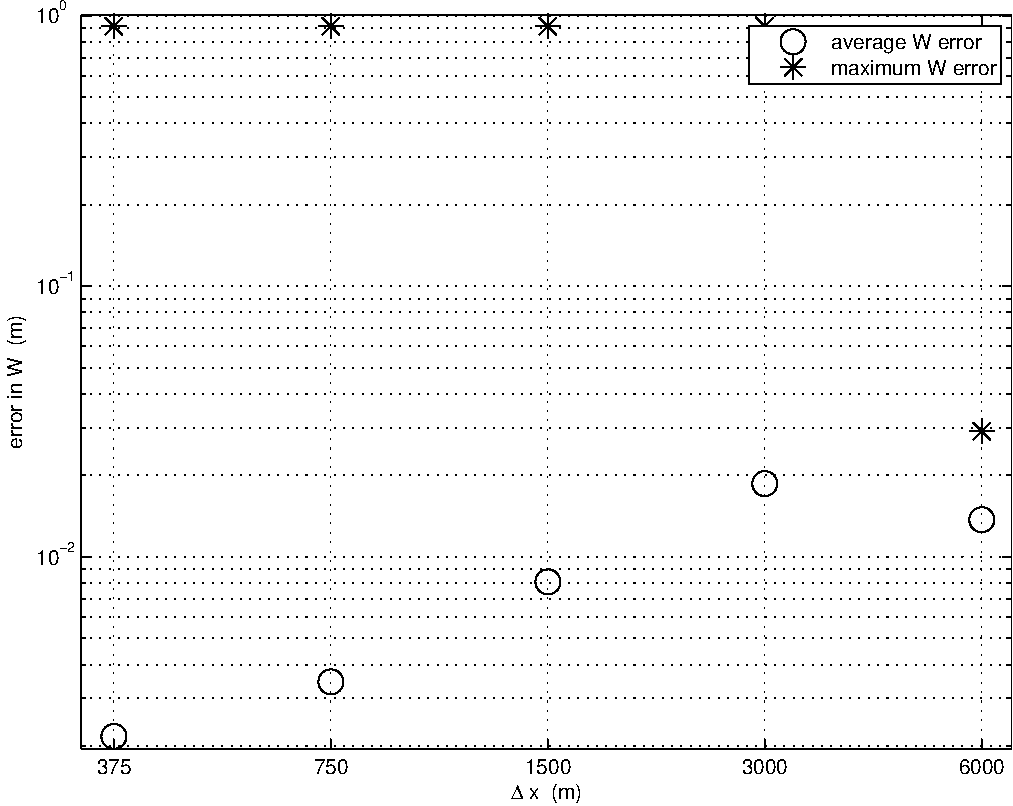
\includegraphics[width=3.5in,keepaspectratio=true]{figs/refineW}
\caption{Average water thickness error $|W-W_{exact}|$ decays with decreasing $\Delta x = \Delta y$.  The average error decays at $O(\Delta x^{0.78})$ for the flux-limited higher resolution scheme (\Large$\circ$\normalsize) and at $O(\Delta x^{0.80})$ the first-order upwind scheme (\scriptsize\,$\square$\,\normalsize).  The maximum errors essentially coincide for the two schemes (\large$\ast$ \normalsize for higher-resolution and $\times$ for first-order).  The maximum error does not decay because of $O(1)$ errors localized at the ice margin.}
\label{fig:refineW}
\end{figure}

\begin{figure}[ht]
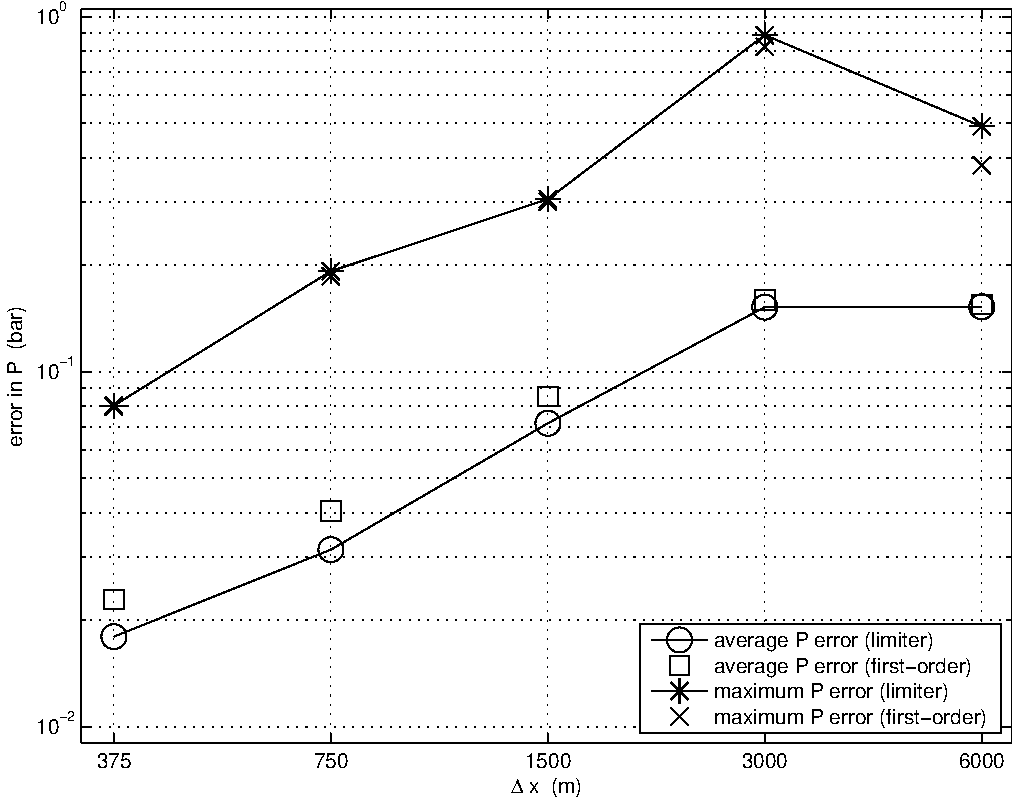
\includegraphics[width=3.5in,keepaspectratio=true]{figs/refineP}
\caption{Average and maximum pressure error $|P-P_{exact}|$ decays with decreasing $\Delta x = \Delta y$.  The average error decays at comparable rates, $O(\Delta x^{1.08})$ for the flux-limited higher resolution scheme (\Large$\circ$\normalsize) and $O(\Delta x^{1.00})$ for the first-order upwind scheme (\scriptsize\,$\square$\,\normalsize).  Again the maximum errors essentially coincide for the two schemes.}
\label{fig:refineP}
\end{figure}

Because they give evidence for numerical convergence, these results suggest that our numerical solution method for these coupled advection-diffusion (for $W$) and diffusion-reaction (for $P$) equations are being solved correctly.  The rate of convergence is not very good, however.  The location of the large errors is entirely in the neighborhood of the ice margin $r=L$ (not shown).  The method for handling boundary conditions is critical to determining the magnitude of the error and its rate of decay.  Further research is needed to decide how to handle this boundary in a more-nearly optimal manner.

The rates of convergence for average errors are nearly identical for the higher resolution flux-limited (Koren) scheme and for the first-order upwinding scheme.  Our problem is a combined advection-diffusion problem in which both the advection velocity and the diffusivity are solution-dependent, and thus it is difficult to separate the errors arising from the numerical treatments of advection and diffusion.  The first-order upwinding scheme for the advection has much larger numerical diffusivity but this diffusivity may be compatible with the continuum model (i.e.~desirable) diffusivity.

Based on this verification evidence, it is reasonable to choose first-order upwinding for applications.  This scheme is simpler to implement, requires fewer floating point operations, and requires a smaller stencil, thus less communication, in a parallel implementation.

As a result of this analysis, only the first-order upwind scheme was implemented in the Parallel Ice Sheet Model (PISM).  Figures \ref{fig:refineWPpism} show results from one month PISM runs using 4 processors on grids with spacing decreasing by factors of two from $5$ km to $156$ m.  This convergence evidence suggests that the PISM implementation is also correct.

\begin{figure}[ht]
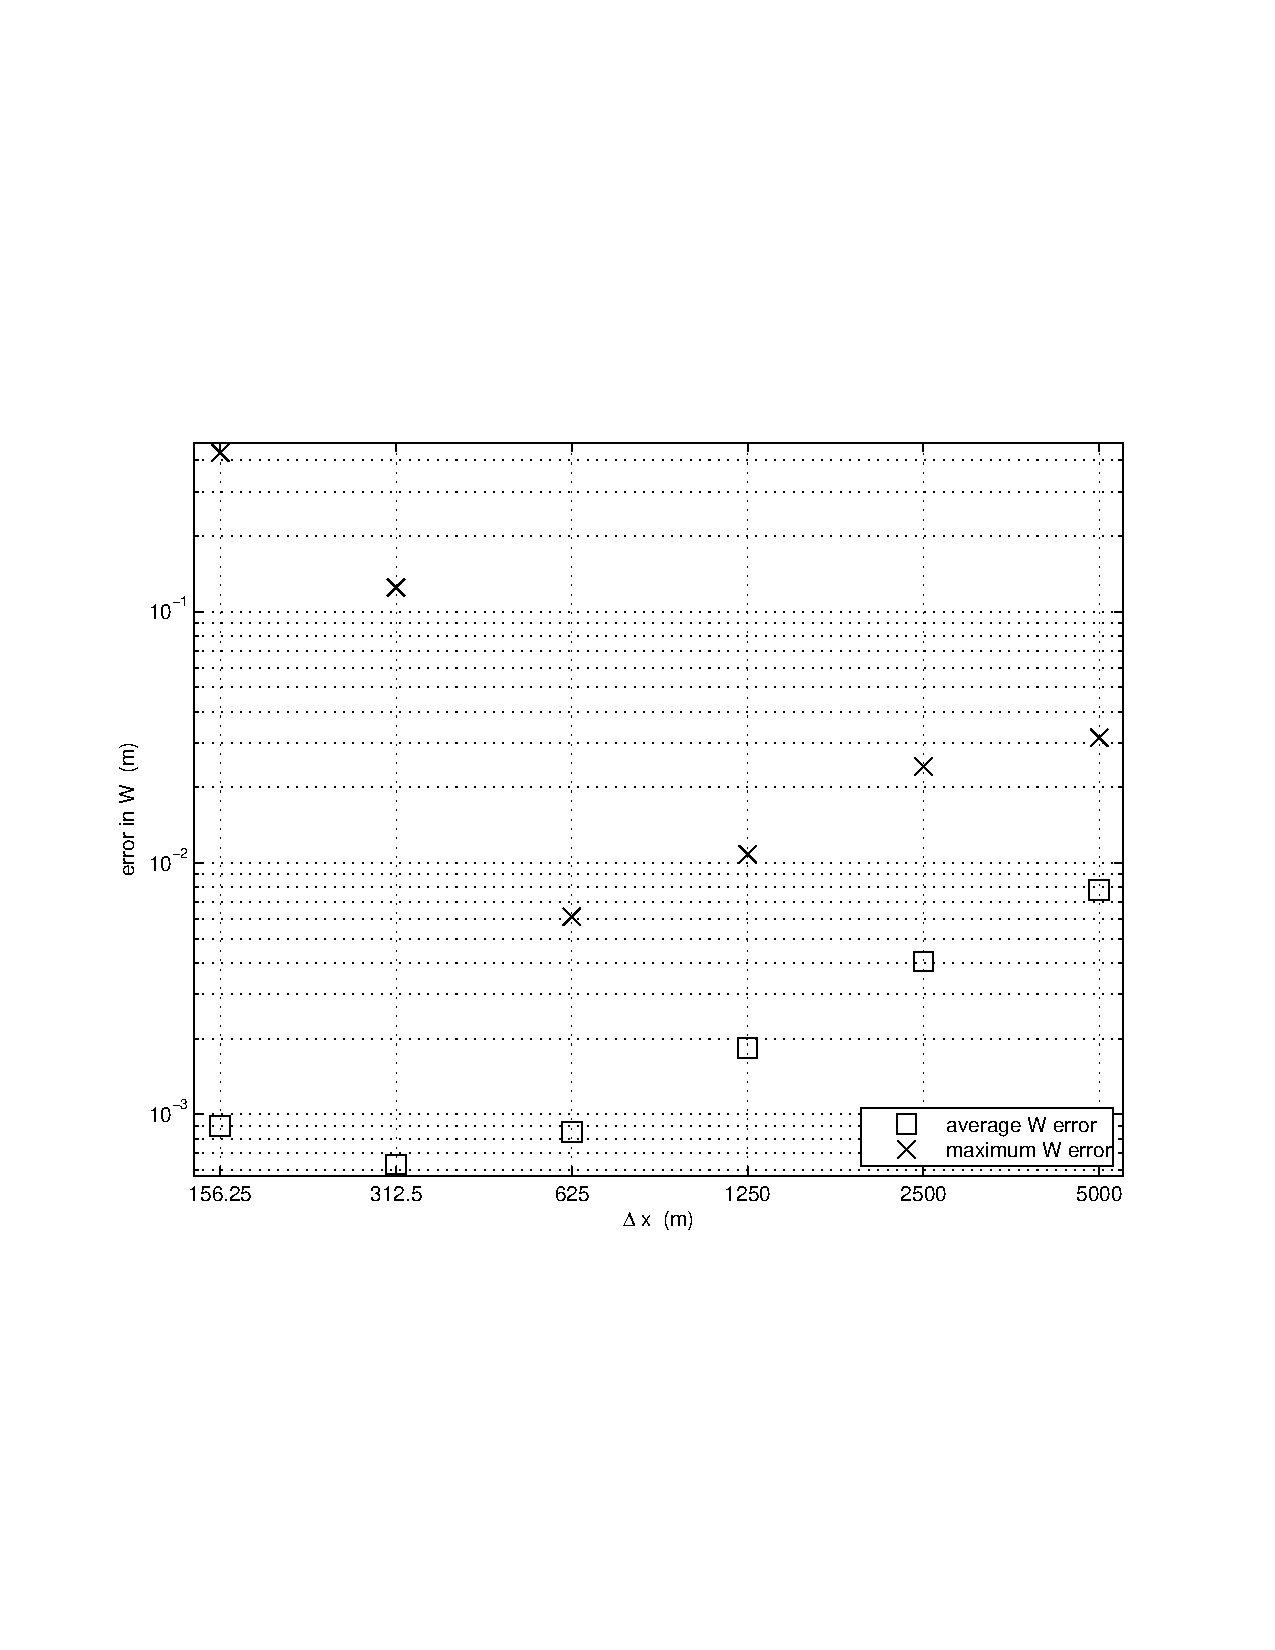
\includegraphics[width=3.0in,keepaspectratio=true]{figs/refineWpism} \quad 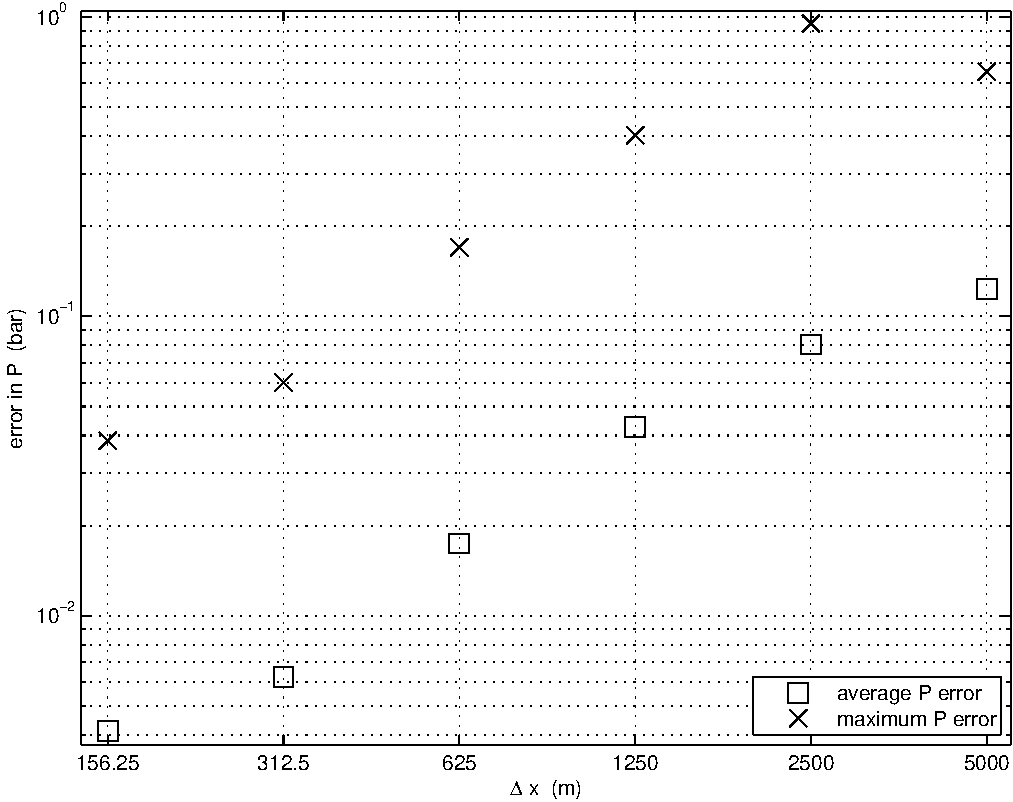
\includegraphics[width=3.0in,keepaspectratio=true]{figs/refinePpism}
\caption{Average water thickness error $|W-W_{exact}|$ decays as $O(\Delta x^{0.85})$ and average pressure error $|P-P_{exact}|$ decays as $O(\Delta x^{1.13})$ in the PISM implementation.}
\label{fig:refineWPpism}
\end{figure}


\subsection*{Steady results for a tidewater glacier}

FIXME: results from nbreen

\begin{figure}[ht]
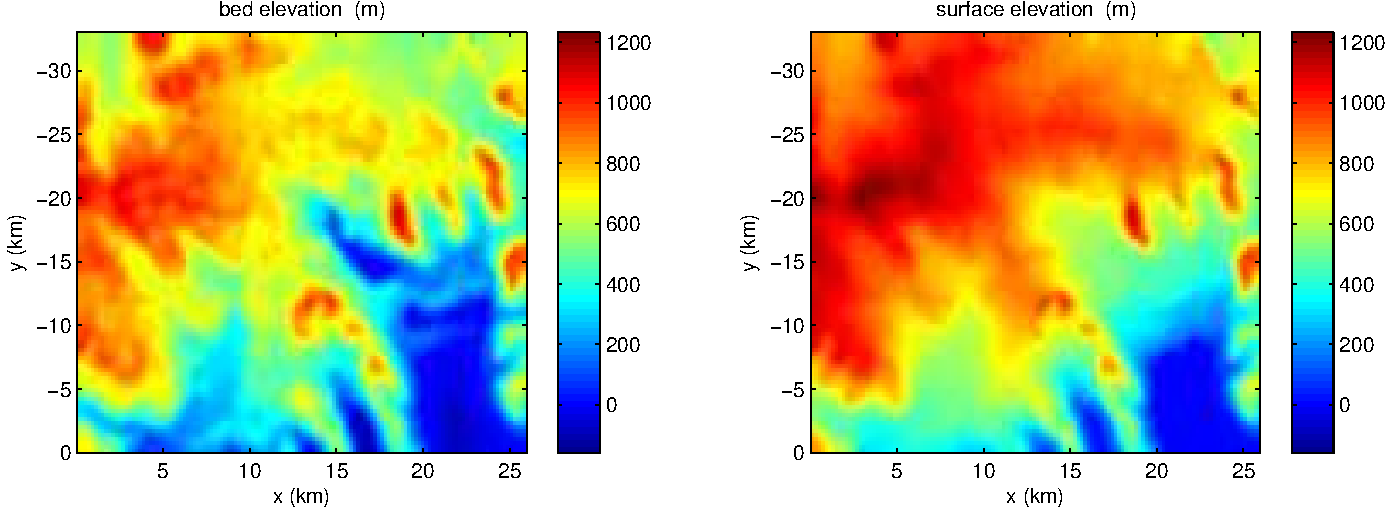
\includegraphics[width=7.0in,keepaspectratio=true]{figs/bed-surf-250m}
\caption{FIXME}
%\label{fig:X}
\end{figure}

\begin{figure}[ht]
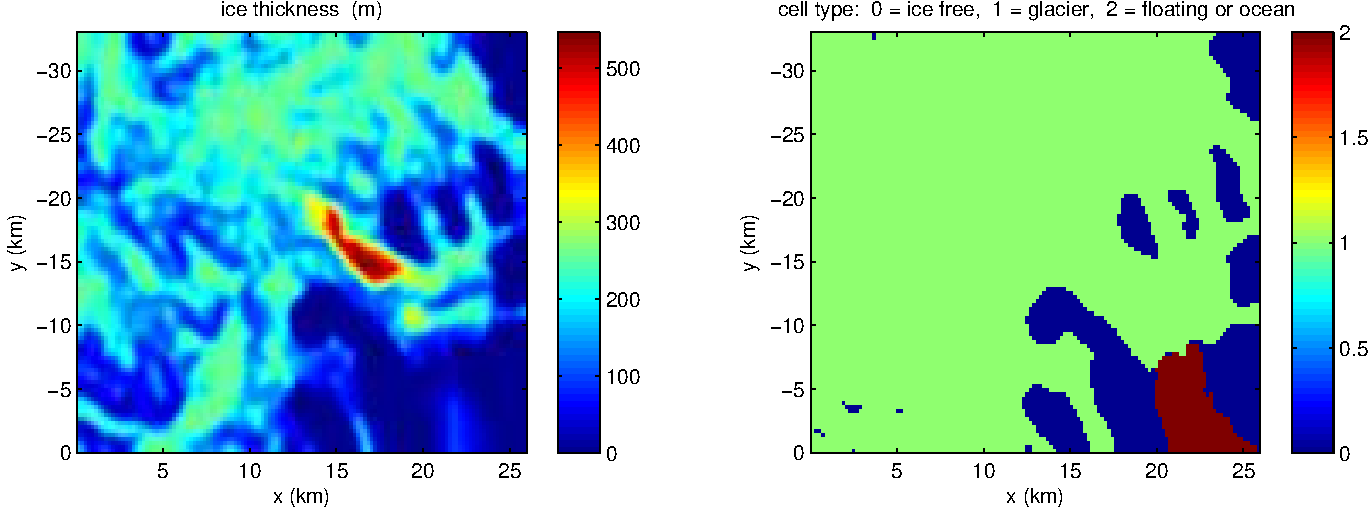
\includegraphics[width=7.0in,keepaspectratio=true]{figs/icethk-icefree-float-250m}
\caption{FIXME}
%\label{fig:X}
\end{figure}

\begin{figure}[ht]
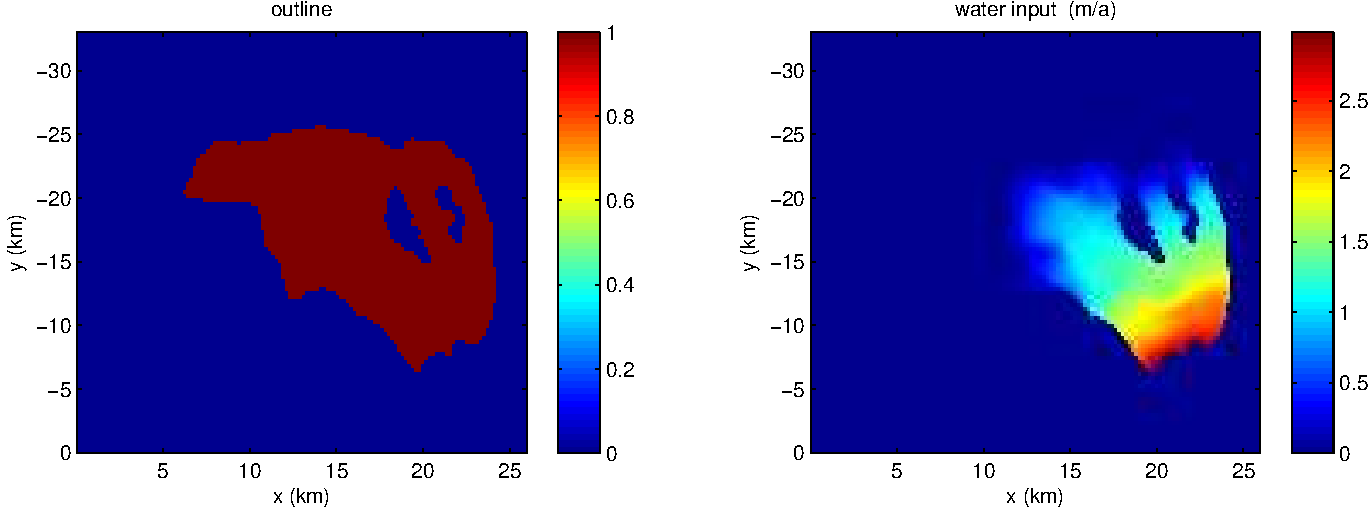
\includegraphics[width=7.0in,keepaspectratio=true]{figs/outline-input-250m}
\caption{FIXME}
%\label{fig:X}
\end{figure}

\begin{figure}[ht]
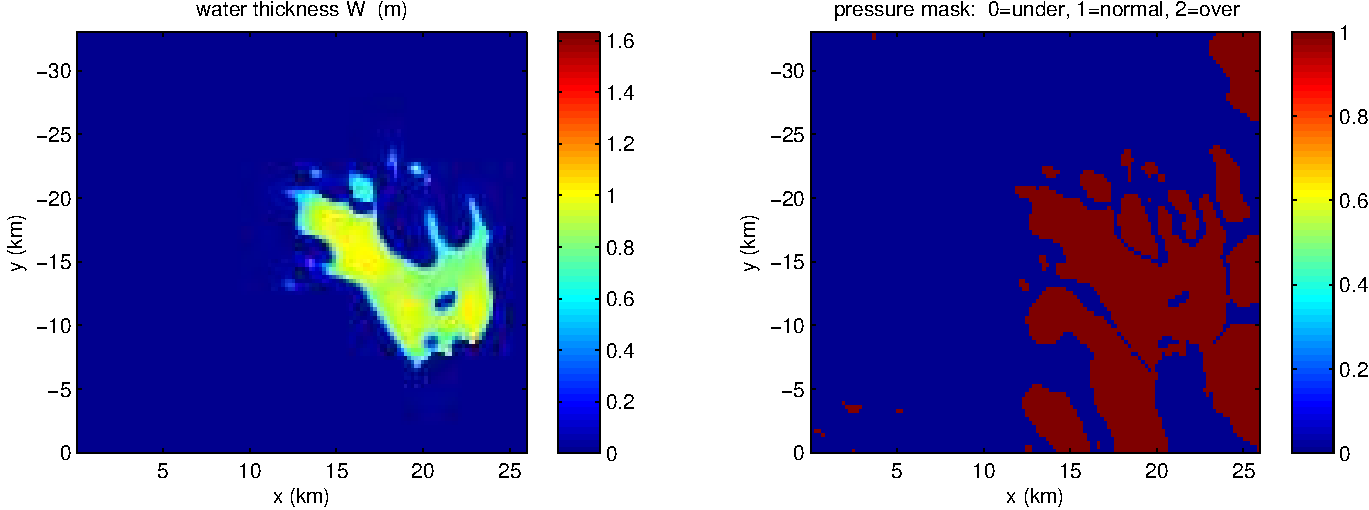
\includegraphics[width=7.0in,keepaspectratio=true]{figs/W-Pmask-250m}
\caption{FIXME}
%\label{fig:X}
\end{figure}

\begin{figure}[ht]
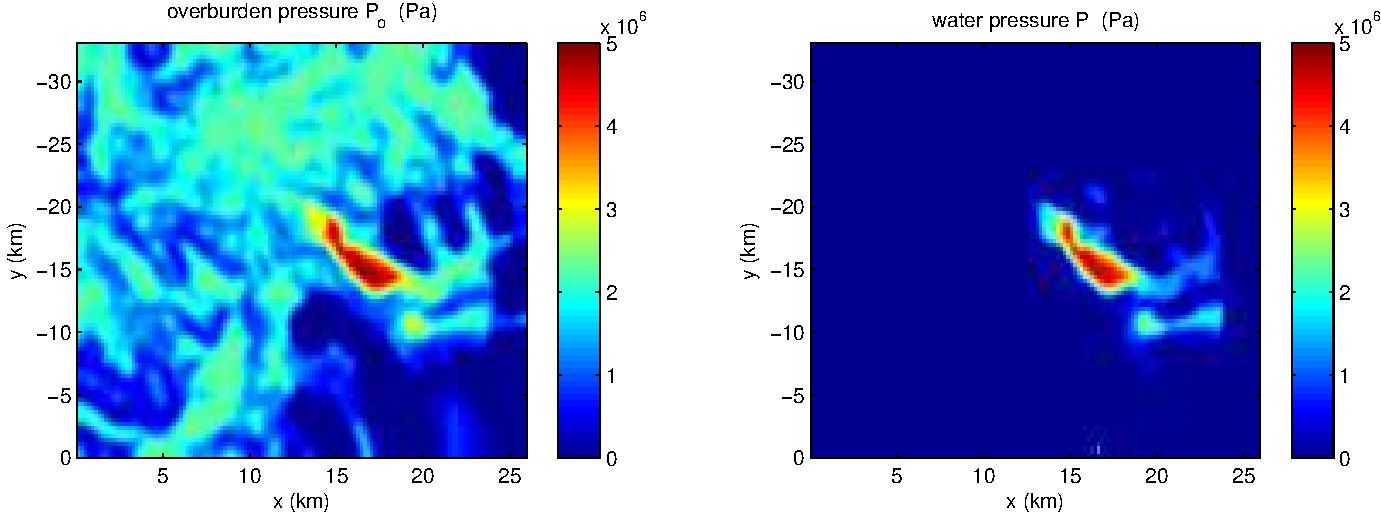
\includegraphics[width=7.0in,keepaspectratio=true]{figs/Po-P-250m}
\caption{FIXME}
%\label{fig:X}
\end{figure}

FIXME:  text about F\&C equation \eqref{eq:PofWFC}

\begin{figure}[ht]
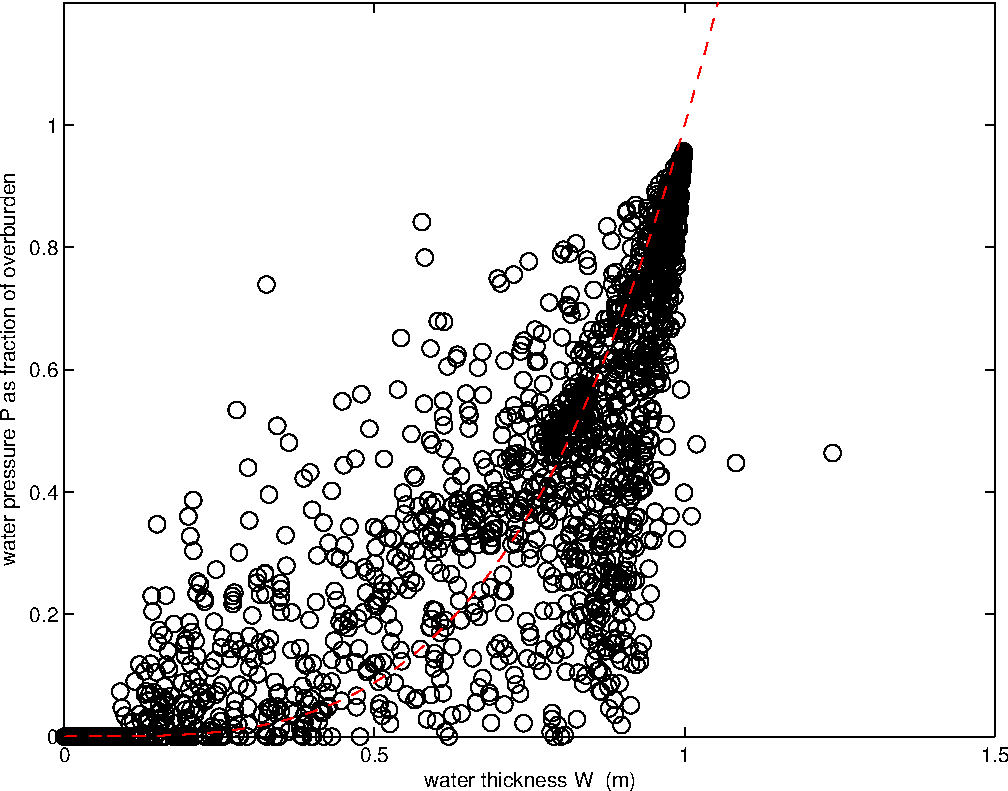
\includegraphics[width=3.0in,keepaspectratio=true]{figs/isPofW-250m} \,
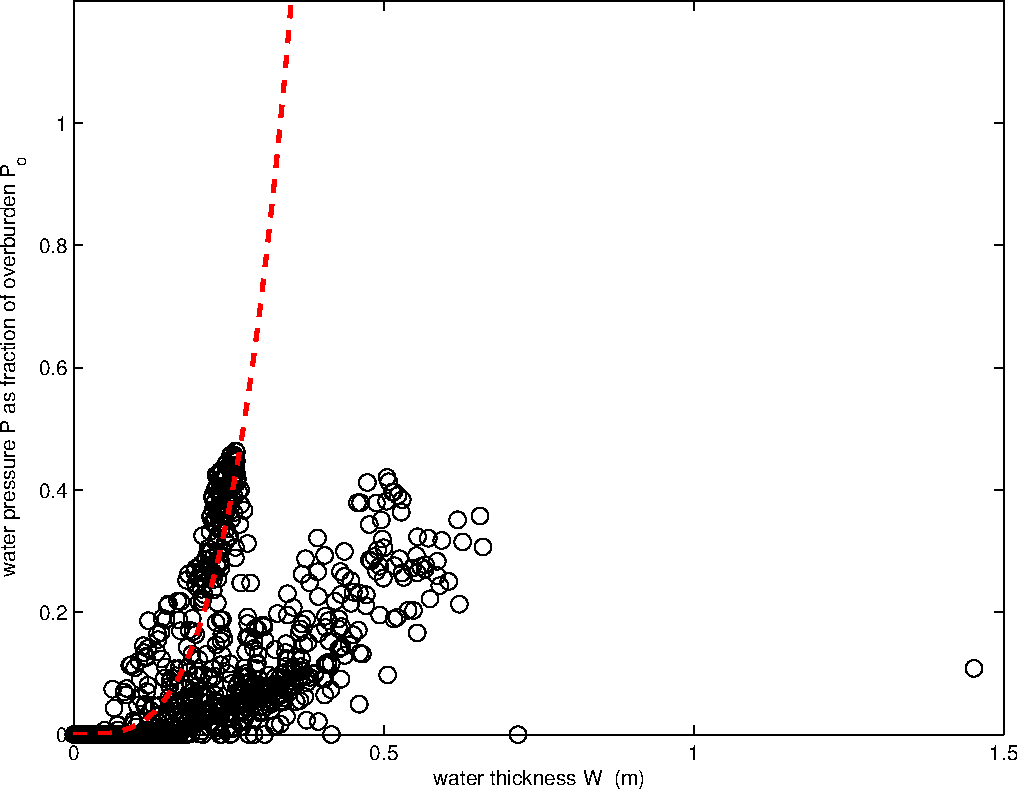
\includegraphics[width=3.0in,keepaspectratio=true]{figs/isPofW-250m-month}
\caption{Left: Scatter plot of $(W,P)$ pairs for all cells at end of 5 year steady-input simulation on a 250 m grid.  Red dashed is equation \eqref{eq:PofWFC} with $W_{\text{crit}} = W_r = 1$ m.  Right: Same except at the end of a one month simulation, and with equation \eqref{eq:PofWFC} using $W_{\text{crit}} = W_r / 3$.}
\label{fig:isPofWnbreen}
\end{figure}


\clearpage\newpage

\small
\bibliography{ice_bib}  % generally requires link to pism/doc/ice_bib.bib
\bibliographystyle{agu}
\normalsize


\clearpage\newpage
\appendix

\section{Positivity and stability of the mass conservation scheme}

Explicit numerical scheme \eqref{eq:Wfd} for the mass conservation PDE \eqref{eq:adeqn}, combined with the first-order upwind case ($\psi=0$) of formulas \eqref{eq:adfluxes}, is sufficiently simple so that we can analyze its properties.  For this scheme we sketch a maximum principle argument \citep{MortonMayers} which shows both stability and positivity (if the water input $\Phi$ is nonnegative and the discrete water thicknesses $\Wlij$ are nonnegative then the updated values $W_{i,j}^{l+1}$ are also nonnegative) for the whole advection-diffusion discretization.    We consider only the case where all of the discrete velocities at the centers of cell interfaces are nonnegative: $\alpha_e\ge 0$, $\alpha_w\ge 0$, $\beta_n\ge 0$, $\beta_s\ge 0$.  The other upwinding cases, wherein these velocity components have various signs, can be handled by similar special-case arguments like the present one.

Let $\nu_x = \Delta t/\Delta x$, $\nu_y = \Delta t/\Delta y$, $\mu_x = K_0 \Delta t / (\Delta x)^2$, and $\mu_y = K_0 \Delta t / (\Delta y)^2$.  We rewrite \eqref{eq:Wfd} as a computation of the next value $W_{i,j}^{l+1}$, and collect terms:
\begin{align*}
 W_{i,j}^{l+1} &= \Wlij - \nu_x \left(\alpha_e \Wlij - \alpha_w W_{i-1,j}^l\right) - \nu_y \left(\beta_n \Wlij - \beta_s W_{i,j-1}^l\right)  \\
      &\qquad + \mu_x \left[W_e \left(W_{i+1,j}^l - \Wlij\right) - W_w \left(\Wlij - W_{i-1,j}^l\right)\right]  \\
      &\qquad + \mu_y \left[W_n \left(W_{i,j+1}^l - \Wlij\right) - W_s \left(\Wlij - W_{i,j-1}^l\right)\right] + \Delta t \Phi_{ij}.
\end{align*}
Rearranging a bit further we get
\begin{align*}
 W_{i,j}^{l+1} &= (\nu_x \alpha_w + \mu_x W_w) W_{i-1,j}^l + (\mu_x W_e) W_{i+1,j}^l + (\nu_y \beta_s + \mu_y W_s) W_{i,j-1}^l + (\mu_y W_n) W_{i,j+1}^l \\
      &\qquad + \Big[1 - \nu_x \alpha_e - \nu_y \beta_n - \mu_x (W_e + W_w) - \mu_y (W_n + W_s)\Big] \Wlij + \Delta t \Phi_{ij}
\end{align*}
so that the new value is a linear combination of the old values, plus a source term:
\begin{equation}
W_{i,j}^{l+1} = A W_{i-1,j}^l + B W_{i+1,j}^l + C W_{i,j-1}^l + D W_{i,j+1}^l + E \Wlij + \Delta t \Phi_{ij}. \label{eq:lincomb}
\end{equation}
Because of our assumption about nonnegative velocities, and assuming $\Wlij \ge 0$ for all $i,j$, we see that coefficients $A,B,C,D$ are all nonnegative, and that only $E$ could be negative.  Thus we can state a sufficient condition based on an equal split between advective and diffusive parts.  Assume a CFL restriction for the advection term in \eqref{eq:adeqn}; this condition generalizes \eqref{eq:CFL}:
\begin{equation}
\nu_x \alpha_e + \nu_y \beta_n = \Delta t \left(\frac{\alpha_e}{\Delta x} + \frac{\beta_n}{\Delta y}\right) \le \frac{1}{2}. \label{eq:adstabcond}
\end{equation}
Also assume a second time-step restriction on the diffusion; compare \eqref{eq:dtDIFFW}:
\begin{equation}
\mu_x (W_e + W_w) + \mu_y (W_n + W_s) = \Delta t \left(\frac{K_0(W_e + W_w)}{\Delta x^2} + \frac{K_0(W_n + W_s)}{\Delta y^2}\right) \le \frac{1}{2}. \label{eq:diffstabcond}
\end{equation}
Thus the coefficient $E$ in \eqref{eq:lincomb} is nonnegative:
	$$E = 1 - \nu_x \alpha_e - \nu_y \beta_n - \mu_x (W_e + W_w) - \mu_y (W_n + W_s) \ge 0.$$
It follows from \eqref{eq:lincomb} that if $\Wlij\ge 0$ and $\Phi_{ij}\ge 0$ for all $i,j$ then $W_{ij}^{l+1}\ge 0$.

We see that all coefficients in linear combination \eqref{eq:lincomb} are nonnegative if the time step restrictions are satisfied.  Furthermore the coefficients add to one.  It follows \citep{MortonMayers} that scheme \eqref{eq:Wfd} with first-order upwinding is positivity-preserving when $\Phi\ge 0$.  It also follows that the scheme is stable under conditions \eqref{eq:dtCFL} and \eqref{eq:dtDIFFW}; these are the all-upwinding-cases generalizations of inequalities \eqref{eq:adstabcond} and \eqref{eq:diffstabcond}, respectively.


\section{Summary of the Bartholomaus et al.~(2011) ``lumped'' model with englacial and subglacial storage}  The model in \cite{Bartholomausetal2011}, which describes the evolution of the intriguing hydrology of the Kennicott glacier in Alaska, is significantly different from the distributed model of \cite{Schoofetal2012} which we focus on in the main text.  On the one hand both of these sources are interested in the relationship of sliding to the evolution of linked-cavity systems, and also both consider physical cavity opening and closing processes.  On the other hand the \cite{Schoofetal2012} theory is distributed and entirely subglacial while the \cite{Bartholomausetal2011} is ``lumped'' (i.e.~the entire glacier is represented by one cell) and there is both subglacial and englacial storage.  In this Appendix we report the equations of the \cite{Bartholomausetal2011} model and derive the pressure evolution equation for this model.  The form of this pressure equation is suggested by equation (12) in \cite{Bartholomausetal2011} but the full pressure equation is not stated.  This pressure equation suggests why we may think of the diffusive regularization \eqref{eq:dampeddstrong} in the main text as actually describing the efficient connection of the subglacial cavity system to englacial storage parameterized by a porosity $\phi$.

The \cite{Bartholomausetal2011} model has the following variables and equations.

The volume of liquid water stored in the glacier is $S(t)$ (m$^3$), and this is split into englacial $S_{en}(t)$ and subglacial $S_{sub}$ portions, thus $S=S_{en}+S_{sub}$.  The cavities have geometry partially-determined by bedrock bumps with cartesian spacing $\lambda_x,\lambda_y$ (m), height $h$ (m), and width $w_c$ (m).  These combine to give a dimensionless capacity parameter $f=(h w_c)/(\lambda_x \lambda_y)$; $f=0.05$ is used for the Kennicott glacier application.  Each cavity has cross-sectional area $A_c$ (m$^2$) so the volume of each cavity is $w_c A_c$ (m$^3$).  The glacier occupies a rectangle of dimensions $L\times W$ in the map-plane so that the number of cavities is $\nu = (LW)/(\lambda_x\lambda_y)$.  It follows that the subglacial storage volume is $S_{sub} = (w_c A_c) \nu = (f L W/h) A_c$.  Englacial water is assumed to fill crevasses and moulins up to a level $z_w$ (m) above the bedrock.  Because the glacier is assumed to have macroporosity $\phi$ (dimensionless), the englacial storage is $S_{en}=L W \phi z_w$.  Mass conservation in the model is the simple statement
\begin{equation}
\frac{dS}{dt} = Q_{in}(t) - Q_{out}(t), \label{eq:barth:massconserve}
\end{equation}
where, in the Kennicott glacier application, both fluxes $Q_{in}$ and $Q_{out}$ are given by measured time-series.

As usual in the current paper, denote the overburden pressure $P_o=\rho_i g H$ and the water pressure $P$ so that $N=P_o-P$ is the effective pressure applied by the glacier to its bed.  The water pressure is fully determined by the amount of englacial storage because there is an assumed efficient connection of the macroporous glacier to it subglacial system.  As the water rises in this system it applies the standard hydrostatic pressure to the subglacier.  Thus
\begin{equation}
P = \rho_w g z_w.  \label{eq:barth:englacialpressure}
\end{equation}

As in the main part of the current paper, the cavity cross-sectional area evolves by physical opening and closure processes.  A wall melt term is also given in \cite{Bartholomausetal2011} but, in keeping with the cavity evolution in the rest of the current paper, we lump it as a melt term $\dot m$.  Denote the sliding speed by $u_b$ and let $C_c = (2 A)/n^n$.  Then the cavity area evolution equation is
\begin{equation}
\frac{dA_c}{dt} = u_b h + \dot m - C_c A_c (P_o-P)^n,  \label{eq:barth:cavityevolution}
\end{equation}
which is a slightly-simplified form of equation (4) in \cite{Bartholomausetal2011}.  The three terms on the right are opening by cavitation, closure by creep, and melt.

We can now write an evolution equation for the pressure.  Starting with equation \eqref{eq:barth:englacialpressure}, and then using $S_{en}=L W \phi z_w$ we can write the pressure rate of change in terms of the englacial storage rate of change:
	$$\frac{dP}{dt} = \rho_w g \frac{dz_w}{dt} = \frac{\rho_w g}{L W \phi} \frac{d S_{en}}{dt}.$$
But the basic fact $S=S_{en}+S_{sub}$ and mass conservation \eqref{eq:barth:massconserve}  allow us to rewrite in terms of fluxes and cavity area:
    $$\frac{dP}{dt} = \frac{\rho_w g}{L W \phi} \left(\frac{d S}{dt} - \frac{d S_{sub}}{dt}\right) = \frac{\rho_w g}{L W \phi} \left(Q_{in} - Q_{out} - \frac{d S_{sub}}{dt}\right).$$
Now use $S_{sub} = (w_c A_c) \nu = (f L W/h) A_c$ to write the evolution in terms of the rate of change of $A_c$:
    $$\frac{dP}{dt} = \frac{\rho_w g}{L W \phi} \left(Q_{in} - Q_{out} - \frac{f L }{h} \frac{d A_c}{dt}\right).$$
Finally incorporate equation \eqref{eq:barth:cavityevolution} to eliminate the derivative $dA_c/dt$:
\begin{equation}
\frac{dP}{dt} = \frac{\rho_w g}{L W \phi} \left(Q_{in} - Q_{out} - \frac{f L }{h} \left[u_b h + \dot m - C_c A_c (P_o-P)^n\right]\right)  \label{eq:barth:fullpressure}
\end{equation}

THE LAST EQUATION FOLLOWS FROM WHAT'S IN BARTH.  IT SUGGESTS HOW TO DISTRIBUTE BARTH, BY RECOGNIZING THAT $(Q_{in} - Q_{out})/L \sim \partial Q/\partial x$.  IT SUGGESTS THAT AT STEADY STATE THE THEORY IN BARTH ALSO HAS $P$ AS A FUNCTION OF $A_c$.  BUT MOST IMPORTANTLY \eqref{eq:barth:fullpressure} IS THE DIRECT ANALOG OF \eqref{eq:dampeddstrong}.  IN FACT, WRITE IT THIS WAY:
\begin{equation}
\frac{\phi}{\rho_w g}\frac{\partial P}{\partial t} = W \left(\frac{\partial Q}{\partial x} - \frac{f}{h} \left[u_b h + \dot m - C_c A_c (P_o-P)^n\right]\right)  \label{eq:barth:pressureanalog}
\end{equation}
THIS EXPLAINS WHY WE REPLACE $E_0/H$ BY $\phi$.



\end{document}
